\documentclass[11pt]{amsart}
\usepackage{geometry,amsmath,amssymb,amsthm,cite,mathtools,float, caption}                % See geometry.pdf to learn the layout options. There are lots.
\usepackage[numbers, sort&compress]{natbib}
\geometry{letterpaper}                   % ... or a4paper or a5paper or ... 
%\geometry{landscape}                % Activate for for rotated page geometry
%\usepackage[parfill]{parskip}    % Activate to begin paragraphs with an empty line rather than an indent
\usepackage{graphicx}
\usepackage{algorithm}
\usepackage[noend]{algpseudocode}
\usepackage{amssymb}
\usepackage{epstopdf}
\usepackage[parfill]{parskip}
\setlength{\parskip}{1ex}
\newtheorem{lemma}{Lemma}
\newtheorem{theorem}{Theorem}
\newtheorem{prop}{Proposition}
\DeclareGraphicsRule{.tif}{png}{.png}{`convert #1 `dirname #1`/`basename #1 .tif`.png}


\title{A compositional model to assess expression changes from
 single-cell RNA-seq data\footnote{Department of Biostatistics and Medical Informatics, UW Madison, Technical Report TR***-v1, May **, 2018.}} 

\author{Xiuyu Ma,  and Christina Kendziorski, and Michael A. Newton}
 
\email{newton@biostat.wisc.edu}
\begin{document}
\maketitle
\section{Introduction}

The ability to measure genome-wide gene expression at single-cell resolution 
has accelerated the pace of biological discovery\cite{scs}.  Overcoming data
analysis challenges caused by the scale and unique variation properties of single-cell
data will surely fuel further advances in immunology\cite{immune}, developmental
biology\cite{dv}, and cancer\cite{cancer} .  Computational tools and statistical methodologies 
created for data of lower-resolution (e.g. bulk RNA-seq) or lower dimension 
(e.g. flow cytometry)  guide our response to 
 the data science demands of new measurement platforms,
but they are not adequate for efficient knowledge discovery in this
rapidly advancing domain\cite{Bacher:2016aa}.

An important feature of single-cell studies that could be leveraged better
statistically is the fact that cells populate distinct, identifiable subtypes
determined by lineage history, epigenetic state, the activity
of various transcriptional programs (e.g. burst states), or other 
distinguishing factors. Lots of efforts have been made to clustering cells
into different cell subtypes, SC3\cite{sc3}, CIDR\cite{CIDR} and ZIFA\cite{ZIFA}.
Whether or not a determination of cellular subtypes and their frequencies 
is a task of interest in a given application, we hypothesize that such
subtype information may be injected into other inferences in order
to improve their operating characteristics.

Assessing the magnitude and statistical significance of changes in gene
expression associated with different cellular conditions has been a central
statistical problem in genomics for which new tools specific to
the single-cell RNAseq data structure have been deployed: MAST\cite{ref:MAST},
DESEQ2\cite{ref:Des}, SCDD\cite{ref:scDD}, etc.  These tools respond
to scRNAseq characteristics, such as high prevelance of zero counts and
gene-level multimodality, but none takes explicit advanatage of cellular subtype
information.  We present a simple procedure and supporting theoretical
analyses for this purpose.  A notable technical innovation is a new prior
distribution over pairs of multinomial probability vectors that conveys
both marginal Dirichlet conjugacy as well as
 dependence induced through sharp equalities on aggregated 
 subtype probabilities, which turns out to be key in formulating 
 the posterior probability of changes in expression distributions between conditions.
 
 
In our compositional model, subtype that inferred from whole genome are fed into gene level expression. 
We utilize the mixture of subtypes to characterize transcripts profile and identify differential distributed genes across conditions in an scRNA-seq experiment.
Simulation study suggests that the method provides improved power and precision for identifying differentially distributed genes. 
Performance on real data has been investigated through ten previously published experimental data from conquer\cite{ref:Cq}. 
We also obtained asymptotic properties of posterior inference. 

\section{Modeling}
\subsection{Data structure, sampling model, and parameters}
In modeling scRNASeq data, we
imagine that each cell $c$ falls into one of $K>1$ classes, which we think of as
subtypes or subpopulations of cells. For notation, $z_c=k$ means that cell $c$ happens to be of subtype $k$, with the vector $z=(z_c)$ recording
the state of all sampled cells.  Knowledge of this class structure
 prior to measurement is not required, as it will be inferred as necessary from
 available genomic data.   We also assume that cells arise from multiple
experimental conditions, such as by treatment-control status or some other factor
 measured at the cell level, and we present our development for the special
case of two conditions.  Notationally, $y=(y_c)$ records the experimental condition, say $y_c=1$ or $y_c=2$ initially:
extensions to multiple conditions are discussed in section 6. Let's say condition $j$ measures $n_j=\sum_{c} 1[y_c=j]$ cells,  and
in total we have $n=n_1+n_2$ cells in the analysis.  Further let $t^j_k = \sum_c 1[y_c=j, z_c=k]$ denote the number of cells of subtype $k$ in condition $j$;
we'll infer something about these counts using genome-wide data.  As for molecular data, the 
normalized expression of gene $g$ in cell $c$, say $X_{g,c}$, is one entry
in a typically large {\sc{genes}} by {\sc{cells}} data matrix $X$.  Summing up, the data structure entails an expression matrix
$X$, a treatment label vector $y$, and a vector $z$ of latent subtype labels.


We treat subtype counts in the two conditions,  $t^1 = (t^1_1, t^1_2, \cdots, t^1_K )$ and 
$t^2 = (t^2_1, t^2_2, \cdots, t^2_K)$,  as independent multinomial
vectors, reflecting the common, two-condition experimental design.  Explicitly,
\begin{eqnarray*}
t^1 \sim \text{Multinomial}_K( n_1, \phi ) \quad {\mbox {\rm and}} \quad
t^2 \sim \text{Multinomial}_K( n_2, \psi )
\end{eqnarray*}
for probability vectors 
$\phi = (\phi_1, \phi_2, \cdots, \phi_K)$ and 
 $\psi = ( \psi_1, \psi_2, \cdots, \psi_K)$ that characterize the populations of
cells from which the $n$ observed cells are sampled.  Our working hypothesis, referred to as the {\em compositional model},  is that any differences in the distribution of expression $X_{g,c}$ 
between $y_c=1$ and $y_c=2$ (i.e., any condition effects) are attributable 
to differences between the conditions 
in the underlying composition of cell types; i.e.,
owing to $\phi \neq \psi$.  We reckon that cells of any given subtype $k$ will
present data according to a distribution reflecting technical 
and biological variation specific to that class of cells, regardless of the 
condition the cell finds itself in.   Some care is needed in this, as an overly
broad cell subtype (e.g. {\em epithelial cells}) could have
further subtypes that show differential response to some treatment, for example,
and so cellular condition (treatment) would then affect the distribution of 
expression data within the subtype, which is contrary to our working hypothesis.
On the other hand, we could then refine the subtype definition to allow more
population classes $K$ in order to mitigate that problem. There's a  risk
 in this approach  if $K$ approaches $n$ (i.e., every cell is it's own type).
In spite of this theoretical possibility, the data sets often encountered 
appear not to display this phenomenon,
even when relatively flexible in the within-subtype expression distribution
We revisit the issue in discussion section, but for now proceed assuming 
that cellular condition affects the composition of subtypes but not the distribution of expression
within a subtype.

With this compositional model, let $f_{g,k}(x)$ denote the sampling distribution
of expression measurement $X_{g,c}$ assuming that cell $c$ is from subtype $k$.
Then in the two cellular conditions, the marginal distributions over subtypes are
\begin{eqnarray*}
f_g^1(x) = \sum_{k=1}^K \phi_k f_{g,k} (x) \quad {\mbox {\rm and}} \quad
f_g^2(x) = \sum_{k=1}^K \psi_k f_{g,k} (x).
\end{eqnarray*}
We say that gene $g$ is {\em differentially distributed}, denote ${\rm DD}_g$,
if $f_g^1(x) \neq f_g^2(x)$ for some $x$, and otherwise it is equivalently distributed
(${\rm ED}_g$). Motivated by findings from bulk RNAseq data analysis, we further
set each $f_{g,k}$ to have a a Negative Binomial form, say with mean $\mu_{g,k}$
and shape parameter $\alpha_g$ (\cite{ref:Leng}; add more citations here). 
This choice proves to be effective in our numerical experiments though it is 
not critical to
the modeling formulation.

We seek a useful methodology to prioritize genes for evidence
of ${\rm DD}_g$.  Interestingly, even if we have evidence for condition effects
on the subtype frequencies, it does not follow that a given
gene will have $f^1_g \neq f^2_g$; that depends on whether or not the subtypes
show the right pattern of {\em differential expression} at $g$, to use the 
standard terminology from bulk RNAseq.  For example, if two subtypes have 
different frequencies between the two conditions ($\phi_1 \neq \psi_1$ and 
 $\phi_2 \neq \psi_2$) but the same aggregate frequency
($\phi_1+\phi_2 = \psi_1 + \psi_2$),  and also  if $\mu_{g,1} = \mu_{g,2}$
then, other things being equal, $f^1_g = f^2_g$ even though $\phi \neq \psi$.
Simply, a gene that does not distinguish two subtypes will also not distinguish
the cellular conditions if those subtypes appear in the same aggregate frequency
in the two conditions, regardless of changes in the individual subtype 
frequencies. We formalize this idea in order that our methodology
has the necessary functionality.  First, consider the parameter space 
\begin{eqnarray*}
\Theta = \{ (\phi, \psi,\mu, \sigma)  \}
\end{eqnarray*}
where $\phi=(\phi_1, \phi_2, \cdots, \phi_K)$ and $\psi=(\psi_1, \psi_2, \cdots, \psi_K)$,
as before, where $\mu = \{ \mu_{g,k} \}$, all the subtype-and-gene-specific expected
values, and where $\sigma = \{ \sigma_g \}$ holds all the gene-specific Negative binomial
shape parameters.  We define special subsets of $\Theta$ using
partitions of the $K$ cell subtypes.  A single partition, say $\pi$, is a set of
mutually exclusive and exhaustive blocks, $b$, say, each a subset of $\{1, 2, 
\cdots, K\}$, and we write $\pi = \{ b \}$.  We recall 
that the set $\Pi$ containing all partitions $\pi$ of $\{1,2, \cdots, K\}$
has cardinality that grows rapidly with $K$. 
 We'll carry along an example
involving $K=7$ cell types, and one three-block partition taken
from the set of 877 possible partitions of $\{1, 2, \cdots, 7\}$ (Figure 1).
\begin{figure}[h!]
%%  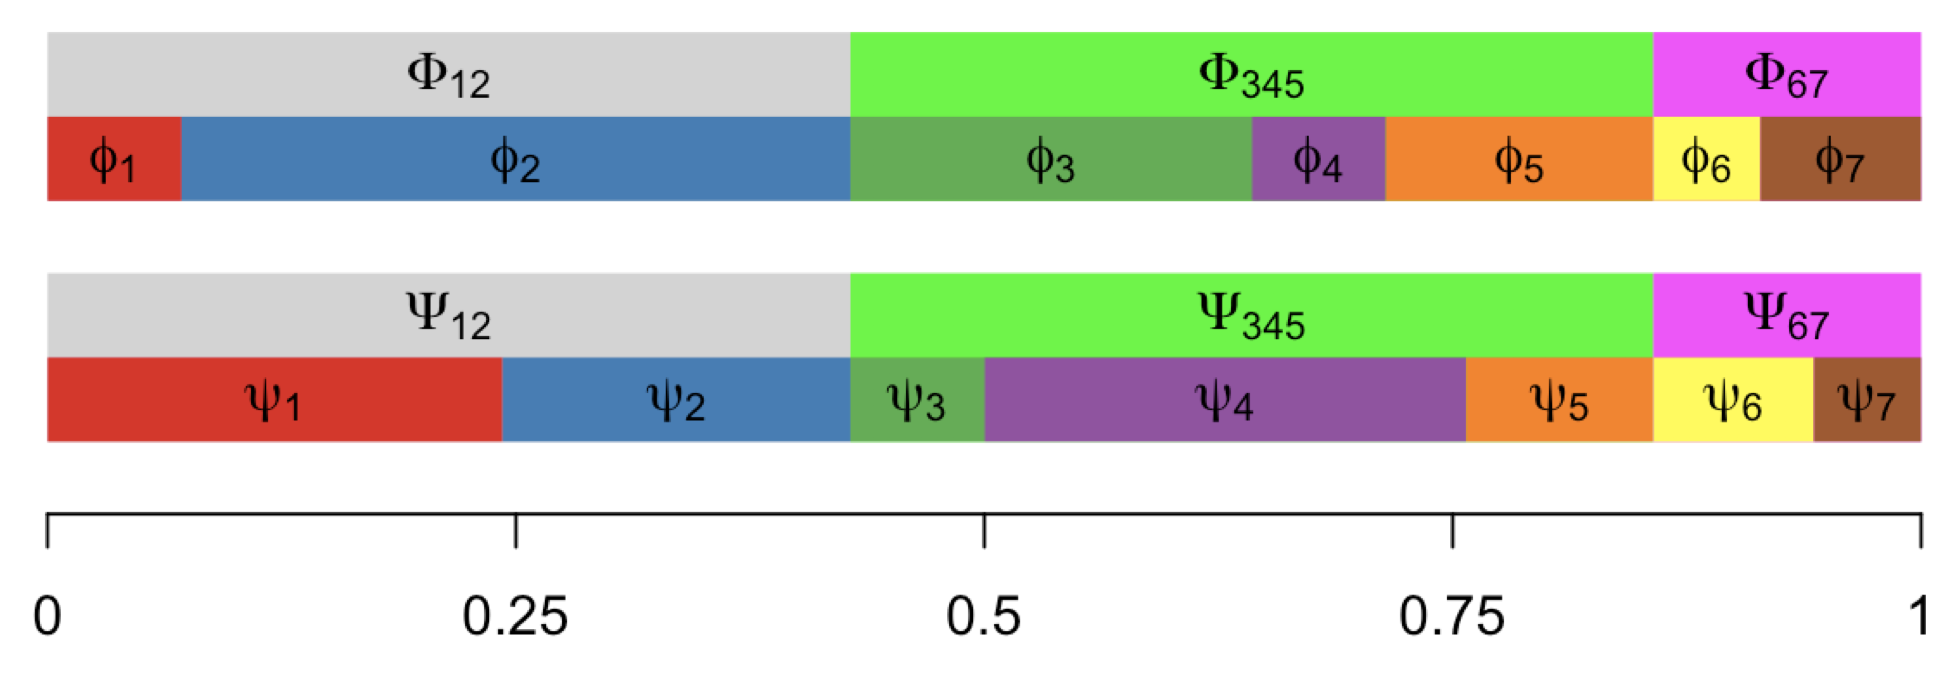
\includegraphics[height = 3.5cm, width=\linewidth]{prop.png}
  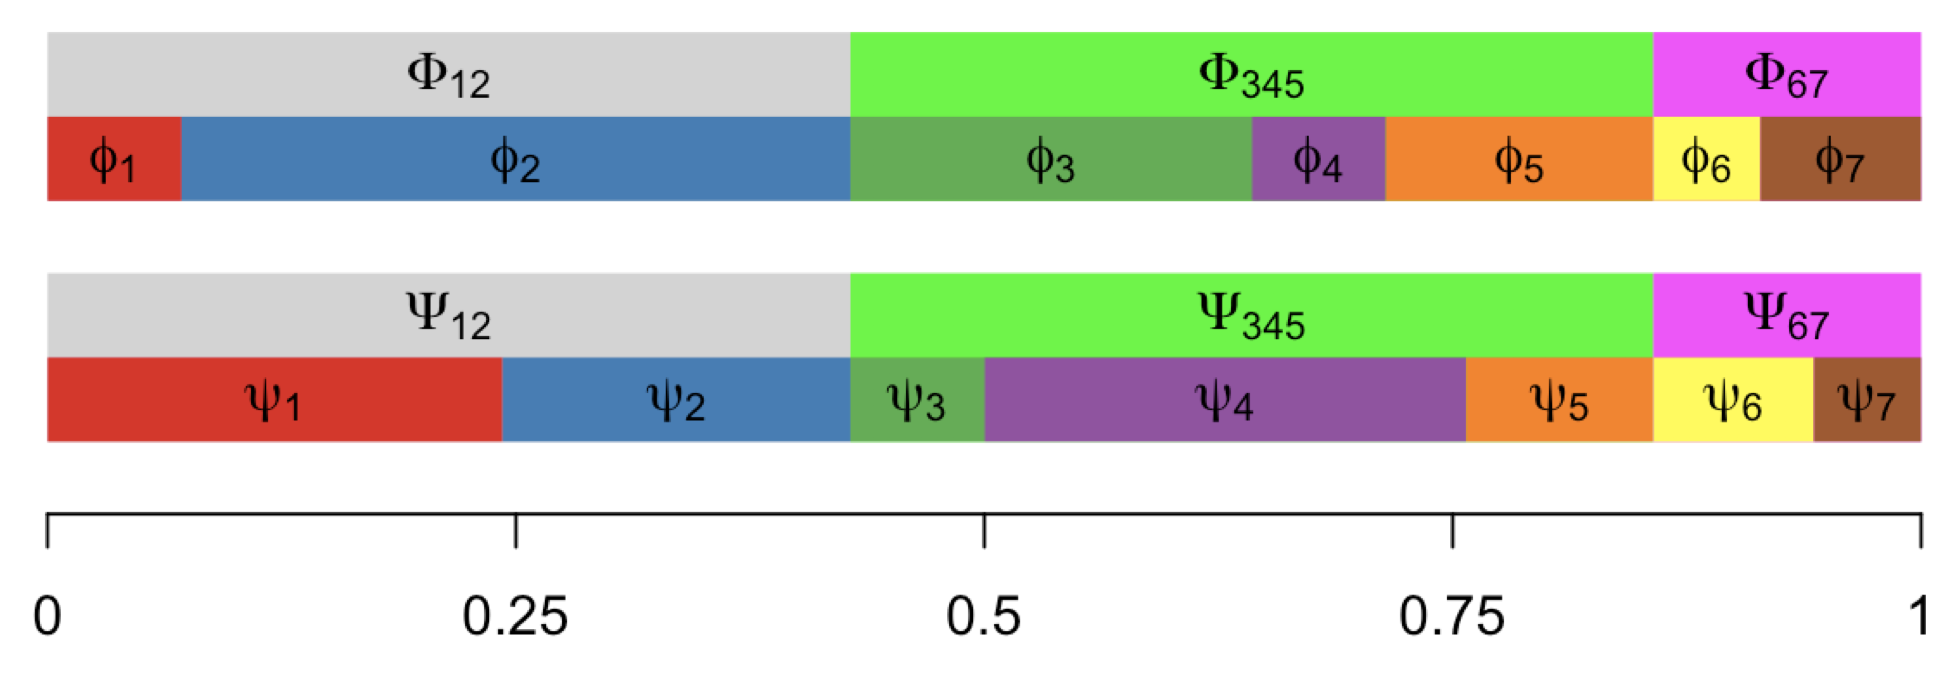
\includegraphics[width=\linewidth]{prop.png}
  \caption{Proportions of $K=7$ cellular subtypes in different conditions. 
 Aggregated proportions of subtype 1 and 2, subtype 3, 4, 5, and subtype 6,7 remained same across conditions while proportion of individual subtype changed. A gene, for example, that shows no differential 
expression between subtypes 1 and 2, and also none among types 3,4, and 5, and none between 6 and 7
 has the same marginal distribution between the two conditions.}
  \label{fig:1}
\end{figure}


For any partition $\pi=\{b\}$ we have aggregate subtype frequencies
\begin{eqnarray*}
\Phi_b = \sum_{k\in b} \phi_k \quad {\mbox {\rm  and}} \quad 
 \Psi_b = \sum_{k\in b} \psi_k.
\end{eqnarray*}
We'll also use the notation $\Phi_\pi = \{ \Phi_b: b \in \pi \}$ and similarly
for $\Psi_\pi$.   As long as $\pi$ is not the most refined partition,
the mapping from $( \phi, \psi )$ to $( \Phi_\pi, \Psi_\pi)$ is many-to-one (Figure 1)
Define
\begin{eqnarray*}
A_\pi = \{ \theta\in \Theta: \; \Phi_b = \Psi_b  \, \forall b \in \pi \}.
\end{eqnarray*}
and
\begin{eqnarray*}
M_{g,\pi} = \{ \theta \in \Theta: \; \mu_{g,k} = \mu_{g,k'} \iff k,k' \in b, b \in \pi \}.
\end{eqnarray*}
Indeed, these are precisely the
structures needed to address differential distribution DD$_g$ (and
it complement, equivalent distribution, ${\rm ED}_g$) at a given gene
$g$: 

\begin{theorem}  Let $C_{g,\pi} = A_\pi\cap M_{g, \pi}$.  For distinct 
partitions $\pi_1,\pi_2$, $C_{g,\pi_1} \cap C_{g,\pi_2} = \emptyset$. Further,
 at any gene $g$, equivalent distribution is
\begin{eqnarray*}
{\rm{ED}}_g = \bigcup_{\pi \in \Pi} C_{g,\pi}.
\end{eqnarray*}
\end{theorem}
 
This representation is central to our empirical Bayes
posterior probabilities, $P(\text{DD}_g|X,y)$, which we develop below, and
which we use to score differential distribution per gene. We require a natural
and simplifying prior assumption:  $A_\pi$ and $M_{g,\pi}$ are independent.
(I.e., proportions $(\phi,\psi)$ are uninformative about the mean expression
  $\{\mu_{g,i}\}$). Then,
\begin{align}
1-P(\text{DD}_g|X,y) = P(\text{ED}_g|X,y) = \sum_{\pi \in \Pi} P(A_\pi|X,y) \,
P(M_{g,\pi}|X).
\end{align}
The idea is by allowing genome-wide information to inform the posterior of $A_\pi$, then get added benefit from the gene-level data, which primarily drives the posterior of $M_{g,\pi}$. It's a very specific form of information sharing that leverages the compositional structure of single-cell data. 

\subsection{Method structure and clustering}



Our approach take transcripts processed by normalizing methods (e.g. SCnorm \cite{ref:Rhonda}). 
The workflow contains two parts, classify cells into subtypes and posterior inference on distributional change. In the first part, recall subtype is a group of cells with distributions of transcripts that are specific to this group, regardless which condition the cells is from. Thus classification process is blind to conditions and can be done by clustering upon similarities between cells(supplementary material). 
\begin{algorithm}
\caption{}\label{alg:scDDboost}
\raggedright\hspace*{\algorithmicindent} \textbf{Input}: Expression data $X$; condition labels $y$; number of cell subtypes $K$ \\
\hspace*{\algorithmicindent} \textbf{Output}: per gene posterior probability of differential distribution
\begin{algorithmic}[1]
\Procedure{scDDboost0}{$X,y,K$}
\State distance matrix: $Dist(X) \gets$ pairwise distances between cells (columns of $X$)
\State cell clustering: $\hat z \gets$ labeled parition of cells, computed from $Dist(X)$ and $K$
\State subtype differential expression: $\forall \pi$,  $P(M_{g,\pi} | X, \hat z)\gets$ using EBSeq\cite{ref:Leng}
\State cell frequency changes: $\forall \pi$, $P(A_\pi | y, \hat z)\gets$ using Double Dirichlet prior
\State posterior probability: $P(\text{ED}_g | X, y, \hat z)\gets \underset{\pi}{\sum}P(M_{g,\pi} | X, \hat z) \,
 P(A_\pi | y, \hat z)$
\State \textbf{return} $P(\text{DD}_g |X, y, \hat z)=1-P(\text{ED}_g| X,y)$
\EndProcedure
\end{algorithmic}
\end{algorithm}

One advantage of our approach is that the posterior inference can be incorporate with different clustering methods. With the development of technology, clustering methods taking care of newly discovered characteristic of scRNA seq data (e.g. SC3\cite{sc3}, CIDR\cite{CIDR} and ZIFA\cite{ZIFA}) could be substituted with our default one. No matter what clustering method is used, we estimate the mixture structure utilizing the whole genome information rather than estimating a gene specific mixture structure solely using information of that gene. Due to this reason, our model is more capable of capturing characteristic of scRNA seq data than scDD and we name our approach scDDboost. 

Although there are various options for clustering methods, none of them guarantee the accuracy and posterior inference can be sensitive to the initial partition. Here we provide a bagging method to make our inferences robust to partitions. Given number of subtypes $K$, the final posterior probabilities is obtained by averaging results from iterative run of scDDboost0 with randomly generated subtype labels $z^*$. Taking account of information contained in $D = Dist(X)$ , instead of purely random assigning subtype labels, we generate the distance matrices of cells $D^*$ by adding noises to the original one and assign labels based on $D^*$. Specifically,  we random sample a noise vector $e$ with length equal to number of cells and components are i.i.d. exponentially distributed. We obtain $D^*$ by adding nosies: $D^* = D + e\textbf{1}^T  + \textbf{1}e^T$. For $D^*$ we still have triangle inequality held as $d_{i,j}^* + d_{j,k}^* \geq d_{i,k}^*$ , it is still a valid distance matrix.
After robustification, we select number of clusters $K$ that posterior probabilities do not vary too much under $K$ and $K+1$.  We validate our procedure in simulated and real data


\begin{algorithm}
\caption{}\label{alg:scDDboost-robust}
\raggedright\hspace*{\algorithmicindent} 
\textbf{Input}: Expression data matrix $X$; condition label vector $y$; number of clusters $K$; \\
\hspace*{\algorithmicindent} number of randomized clusterings $n_r$; regularization parameter $\lambda$   
\\
\hspace*{\algorithmicindent} \textbf{Output}: per gene posterior probability of differential distribution 
\begin{algorithmic}[2]
\Procedure{scDDboost1}{$X,y, K, n_r, \lambda$}
\State distance matrix: $D=Dist(X) \gets$ pairwise distances between cells (columns of $X$)
\Repeat
\State Exponential noise vector: $e$, with components $\sim \text{Exp}(\lambda)$
\State randomized distance matrix: $D^* \gets D + e\textbf{1}^T +  \textbf{1}e^T$
\State cell clustering: $z^* \gets$ labeled parition of cells, computed from $D^*$ and $K$
\State subtype differential expression: $\forall \pi$,  $P(M_{g,\pi} | X, z^*)\gets$ using EBSeq\cite{ref:Leng}
\State cell frequency changes: $\forall \pi$, $P(A_\pi | y, z^*)\gets$ using Double Dirichlet prior
\State posterior probability: $P(\text{ED}_g | X, y, z^*)\gets \underset{\pi}{\sum}P(M_{g,\pi} | X, z^*) \,
 P(A_\pi | y, z^*)$
\Until{$n_r$ randomized clusterings $z^*$}
\State \textbf{return} $1-\frac{1}{n_r} \sum_{z^*} P(\text{ED}_g |X, y,z^*)$
\EndProcedure
\end{algorithmic}
\end{algorithm}

**needs further refinement**
After identification of subtypes, the second part of our procedure involving two steps use empirical Bayes to provide posterior inference on patterns of differential expression($M_{g,\pi}$) and aggregated proportions of subtypes($A_\pi$), where $P(M_{g,\pi} | X)$ is done in EBSeq\cite{ref:Leng} and we present details of calculating $P(A_\pi | X)$ in next section. Combining those components, final posterior probabilities are obtained. 


\section{Empirical Bayes}
\subsection{Double Dirichlet prior}

Here we describe a prior $p(\phi,\psi)$ that is conjugate to multinomial
sampling but that also enables downstream gene-specific inferences about
differential distribution when certain 
cell types do not differ in their expression
distributions.  


For our purposes, the prior will have a spike-slab structure that mixes
over distinct patterns of equality of $\pi$-associated
accummulated probabilities:
\begin{eqnarray*}
p(\phi,\psi) = \sum_{\pi \in \Pi} P(A_\pi) \, p(\phi,\psi| A_\pi )
\end{eqnarray*} 
Upon setting up a prior $p(\phi,\psi)$ that can mix over structures
$A_\pi$, we can obtain posterior inference $P(A_\pi | t^1, t^2)$

Initially, the multitude of $P(A_\pi)$'s will be preset constants.To complete the prior specification $p(\phi,\psi)$, consider further scalers
$\alpha_k>0$ for each class $k$ and $\beta_b>0$ for each potential block $b$.
(Extending the notational convention, $\alpha_b$ is the vector of $\alpha_k$
for $k\in b$, and $\beta_\pi$ is the vector of $\beta_b$ for $b \in \pi$.)
For any block $b$ consider conditional probabilities
\begin{eqnarray*}
\tilde{\phi}_b = \frac{\phi_b}{\Phi_b} \qquad \tilde{\psi}_b = \frac{\psi_b}{\Psi_b}
\end{eqnarray*}
which indicate the conditional probability of each class $k$ given that
the cell is of one of the types in $b$.  Assume that conditional upon 
$A_\pi$,
\begin{eqnarray*}
\Phi_\pi \sim \text{Dirichet}_{N(\pi)}[   \beta_\pi   ]
\end{eqnarray*}
where $N(\pi)$ is the number of blocks $b$ in $\pi$,
and further that accumulated probabilities are the same between
the two source conditions: $\Phi_\pi = \Psi_\pi$.
Finally, assume that for each $b \in \pi$,
\begin{eqnarray*}
\tilde \phi_b, \tilde \psi_b \sim_{\text{i.i.d.}}
  \text{Dirichlet}_{N(b)}[ \alpha_b ]
\end{eqnarray*}
where $N(b)$ is the number of cell types in block $b$.
In other words, if $A_\pi$ is the active structure, then
accumulated probability vectors $\Phi_\pi$ and $\Psi_\pi$ are equal
between the two source conditions, though the sub-block class-specific
rates $\phi_k$ and $\psi_k$ may differ, as would (re-normalized)
independent Dirichlet-distributed vectors.
Taken together,
\begin{eqnarray*}
p(\phi,\psi|A_\pi) =
         p( \Phi_\pi, \Psi_\pi | A_\pi ) \, \prod_{b \in \pi}  \left[
         p( \tilde \phi_b ) p( \tilde \psi_b ) \right]
\end{eqnarray*}
with
\begin{eqnarray*}
p( \Phi_\pi, \Psi_\pi | A_\pi )
= \frac{\Gamma(\sum_{b\in \pi} \beta_b)}{
 \prod_{b \in \pi} \Gamma( \beta_b )} \left[\prod_{b \in \pi} \Phi_b^{\beta_b-1} \right] \,
 1\left[ \Phi_\pi = \Psi_\pi \right]
\end{eqnarray*}
and
\begin{eqnarray*}
p( \tilde \phi_b ) =
\frac{ \Gamma( \sum_{k\in b} \alpha_k ) }{ \prod_{k\in b} \Gamma(\alpha_k) }
 \prod_{k \in b} \tilde \phi_k^{\alpha_k -1 },
\qquad
p( \tilde \psi_b )
=
\frac{ \Gamma( \sum_{k\in b} \alpha_k ) }{ \prod_{k\in b} \Gamma(\alpha_k) }
\prod_{k \in b} \tilde \psi_k^{\alpha_k -1 }.
\end{eqnarray*}



\subsection{Predictive probabilities:}
For notation, we use $\phi_b$ for the vector of values $\phi_k$ for $k \in b$,
and similarly for $\psi_b$. Analogously, $\Phi_\pi$ and $\Psi_\pi$
 are vectors of 
accumulated class probabilities $\phi_b$ and $\psi_b$ for all $b \in \pi$,
 respectively. \\
In order to get the posterior probability $p(A_\pi | t^1,t^2)$, we need to calculate 
\[
\begin{split}
p(A_\pi | t^1,t^2)\propto p(A_\pi, t^1,t^2) &= \int_{A_\pi} p(t^1,t^2|\phi,\psi)p(\phi,\psi) d\phi d\psi\\ 
&= \sum_{\pi'\in \Pi}\int_{A_\pi} p(t^1,t^2|\phi,\psi)p(\phi, \psi | A_{\pi'})p(A_{\pi'})d\phi d\psi
\end{split}
\]
For simplicity of notation, let $w(\pi_1, \pi_2) = \int_{A_{\pi_1}} p(t^1,t^2|\phi,\psi)p(\phi, \psi | A_{\pi_2})p(A_{\pi_2})d\phi d\psi$, then 
$p(A_\pi | t^1,t^2)\propto \underset{\pi'\in \Pi}\sum w(\pi, \pi')$. To calculate component $w(\pi, \pi')$, recall refinement and coarseness relationship between partitions, we say a partition $\tilde{\pi}$ is a refinement of another partition $\pi$ if $\forall b \in \pi$ there exists $s \subset \tilde{\pi}$  such that $\underset{b'\in s}\cup b' = b$. We say $\pi$ is a coarseness of $\tilde{\pi}$ when $\tilde{\pi}$ refines $\pi$. we have following theorem

\begin{theorem}
If $\pi'$ is a refinement of $\pi$ then $w(\pi,\pi') = w(\pi', \pi')$ otherwise $w(\pi,\pi') = 0$
\end{theorem}
\hfill\\
Consequently, let $RF(\pi)$ be the collection of finer partition of $\pi$, we have 
the posterior probability: 
\[
\begin{split}
p(A_\pi | t^1,t^2)\propto  \sum_{\pi' \in RF(\pi)} w(\pi',\pi')
\end{split}
\]
Using the Dirichlet-Multinomial conjugacy and the collapsing property of
these distributions (\cite{ref:Dickey}), we get closed formulas for the predictive
probability of cell-type counts $t^1$ and $t^2$.  Fixing $\pi$,
let $t^j_b = \sum_{k\in b} t^j_k$, for cell conditions $j=1,2$, 
record the total numbers of cells accumulated over all types in block $b$.
And following our notation convention, $t^j_\pi$ is the vector of these
counts over $b \in \pi$.  From the prior and model structure
\begin{eqnarray*}
w(\pi, \pi) = p(t^1 | t^1_{\pi})\, p(t^2|  t^2_{\pi} )
 \, p( t^1_{\pi}, t^2_{\pi} | A_{\pi} ) p(A_{\pi}).
\end{eqnarray*}
Conditional independence of $t^1$ and $t^2$ given the block-level totals
$t^1_{\pi}$ and $t^2_{\pi}$ on $A_{\pi}$ reflects the possible differential 
class proportion structure within blocks but between cell conditions.
For either cellular group $j=1,2$,
we find, after some simplification, the following Dirichlet-Multinomial masses: 
\begin{align}
p(t^j | t^j_{\pi}) = \prod_{b \in \pi} \left\{
\left[ \frac{ \Gamma(t^j_b +1 ) }{\prod_{k \in b} \Gamma( t^j_k + 1 ) } 
\right]
\left[ \frac{\Gamma( \sum_{k \in b} \alpha_k )}{
		\prod_{k\in b} \Gamma( \alpha_k ) } \right] 
       \left[        \frac{ \prod_{k \in b} \Gamma(\alpha_k + t^j_k)  }{
		\Gamma(t^j_b + \sum_{k\in b} \alpha_k ) )}\right]
 \right\}
\end{align}
and
\begin{align}
p(t^1_{\pi},t^2_{\pi}| A_{\pi}) =
 \left[ \frac{ \Gamma(n_1+1) \Gamma(n_2+1) }{ \prod_{b \in \pi} \Gamma(t^1_b+1) 
   \Gamma( t^2_b + 1 )} \right] 
\left[ \frac{\Gamma( \sum_{b \in \pi} \beta_b  )}{
   \prod_{b \in \pi} \Gamma(\beta_b )} \right] 
 \left[ \frac{ \prod_{b \in \pi} \Gamma( \beta_b + t^1_b + t^2_b )}{
	\Gamma( n_1 + n_2 + \sum_{b \in \pi} \beta_b  )} \right].
\end{align}
\hfill\\
Let's look at some special cases to dissect this result. \\
Case 1. If $\pi$ has a single block equal to the entire
 set of cell types $\{1,2, \cdots, K\}$,  then $t^j_b=n_j$ for both $j=1,2$,
and the second formula reduces, correctly, to 
$p(t^1_{\pi},t^2_{\pi}| A_{\pi}) = 1$.  Further,
\begin{eqnarray*}
p(t^j | t^j_{\pi}) = 
\left[ \frac{ \Gamma(n_j +1 ) }{ \Gamma( n_1 + \sum_{k=1}^K \alpha_k ) }
\right]
\left[ \frac{\Gamma( \sum_{k =1}^K \alpha_k )}{
                \prod_{k=1}^K \Gamma( \alpha_k ) } \right]
       \left[    \prod_{k=1}^K    \frac{  \Gamma(\alpha_k + t^j_k)}{
                \Gamma(t^j_k + 1 )}\right]
\end{eqnarray*}
which is the well-known Dirichlet-multinomial predictive distribution
for counts $t^j$ \cite{Wag}.  E.g, taking $\alpha_k=1$ for all types $k$ 
we get the uniform distribution
\begin{eqnarray*}
p(t^j | t^j_{\pi}) = 
 \frac{ \Gamma(n_j +1 ) \Gamma(K) }{ \Gamma( n_j + K ) }.
\end{eqnarray*}
Case 2. At the opposite extreme, $\pi$  has one block $b$ for each
 class $k$. Then $t^j_b = z^j_k$, and $p(t^j | t^j_{\pi}) = 1$, and 
further, assuming $\beta_b = \alpha_k$,
\begin{eqnarray*}
p(t^1_{\pi},t^2_{\pi}| A_{\pi}) =
 \left[ \frac{ \Gamma(n_1+1) \Gamma(n_2+1) }{ \prod_{k=1}^K 
   \Gamma(t^1_k+1) 
   \Gamma( t^2_k + 1 )} \right] 
\left[ \frac{\Gamma( \sum_{k=1}^K \alpha_k  )}{
   \prod_{k=1}^K \Gamma(\alpha_k )} \right] 
 \left[ \frac{ \prod_{k=1}^K \Gamma( \alpha_k + t^1_k + t^2_k )}{
	\Gamma( n_1 + n_2 + \alpha_k  )} \right].
\end{eqnarray*}
which corresponds to Dirichlet-multinomial predictive distribution for counts $t^1 + t^2$ 
since $t^1$ and $t^2$ are identical distributed in this case.

Regardless of the partition,
log scale probabilities are readily evaluated 
given hyper-parameters $\{ \alpha_k \}$ and $\{ \beta_b \}$ and for
cell-type counts $t^1$ and $t^2$. \\
For asymptotic properties of the posterior probabilities, we demonstrated them in section 6. 
 
\section{Simulation study} 

A simulation study was conducted to assess the performance of
scDDboost in identifying DD genes.
We simulate data by splatter\cite{ref:Zappia} with approximate 200 cells each condition and 7 subtypes with proportions $\phi$ and $\psi$ from Figure 1 satisfying constraints: $\phi_1 + \phi_2 = \psi_1 + \psi_2$, $\phi_3 + \phi_4 +\phi_5 = \psi_3 + \psi_4 + \psi_5$ and $\phi_6 + \phi_7 = \psi_6 + \psi_7$. Each subtype has 10\% genes to be differential expressed. We view the differences among subtypes by projecting transcripts profiles of cells into its first two principal components(figure 2). We observed subtypes are well separated, which is driven by genes with heterogeneous distribution between subtypes. 
\begin{figure}[h!]
  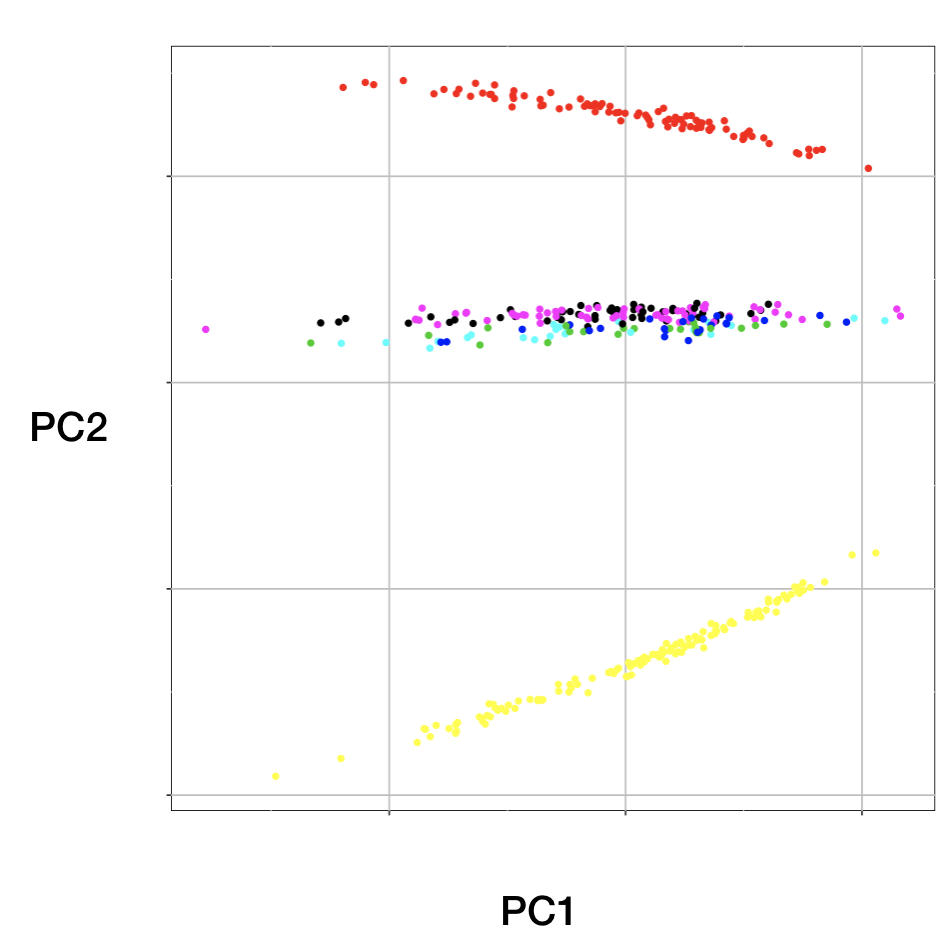
\includegraphics[ width = 0.4\textwidth]{pca.png}
  \caption{first two principal components of transcripts, which demonstrates the difference between subtypes. Even if we projected transcripts of cells into two dimensional space, we observe subtypes are well separated.}
  \label{fig:4}
\end{figure}

We determine the number of subtypes by searching a range of candidates(from 1 to 9 based on our empirical experience). Given number of subtypes, we obtain a subtype structure of cells, which will further be fed into computing the posterior probabilities. We visualize the change between posterior probabilities under number of clusters $i$ and $i + 1$($i$ from 1 to 8). It typically remains stable when number of cluster is above a number that is smaller than 9 (figure 3)
In the simulated data, the posterior probability become stable when we overestimate the number of subtypes. We found the true number of subtypes is 7 and correctly identify the subtypes of cells.   

10\% DE genes in each subtype results in total 8704 DD genes and 8669 ED genes in the mixture of the 7 subtypes.
Table 1 are numbers of DD or DE genes identified by four methods (scDDboost, scDD, MAST and DESeq2) with target FDR at 5 \%. 
\begin{table}
\centering
\begin{tabular}{ |p{3cm}|p{2cm}|p{2cm}|p{2cm}|p{2cm}|}
\hline
 & scDDboost & scDD & MAST & DESeq2\\
\hline
\hline
DD or DE genes & 5126 & 1593 & 2559 & 3000\\
\hline
True positive & 5094 & 1570 & 2508 & 2928\\
\hline
false positive & 32 & 23 & 51 & 72\\
\hline
\end{tabular}
\captionof{table}{number of true positive and false positive genes identified by four methods. Target FDR at 5\%}
\end{table}


scDDboost identified most true DD genes, the reason is that mean expression shifts between conditions is not as significant as mean expression shifts between subtypes, which limits the power of MAST and DESeq2. Our approach and scDD considered mixture structure underlying the transcrips but scDD did not use the whole genome information to infer mixture components, which leads to inaccurate clustering at gene level and reduce the power. Under randomized distance, scDDboost gave an accurate estimation of subtypes and thus are more sensitive to the mean expression change among subtypes. We also compare roc curves of scDDboost, scDD, MAST and DESeq2. (figure 4)
\begin{figure}[h]
\vspace{-\parskip}
\minipage{0.5\textwidth}
  \includegraphics[width=\textwidth]{sim_67.png}
\endminipage\hfill
\minipage{0.5\textwidth}
  \includegraphics[width=\textwidth]{sim_78.png}
  \endminipage
\caption{comparison of posterior probabilities of being DD among different number of subtypes, when we underestimate the number of subtypes, the difference is huge, see PDD between 6 subtypes and 7 subtypes. There is an approximate horizontal line with massive points at the top of left panel, which indicate that we underestimate lots of DD genes due to underestimate the number of subtypes. While in the case when we overestimate the number of subtypes 7 subtypes vs. 8 subtypes, though inflating PDD but the variation of difference is small, from 6 to 8 subtypes the PDD become more linear related.}
\end{figure}
\begin{figure}[H]
  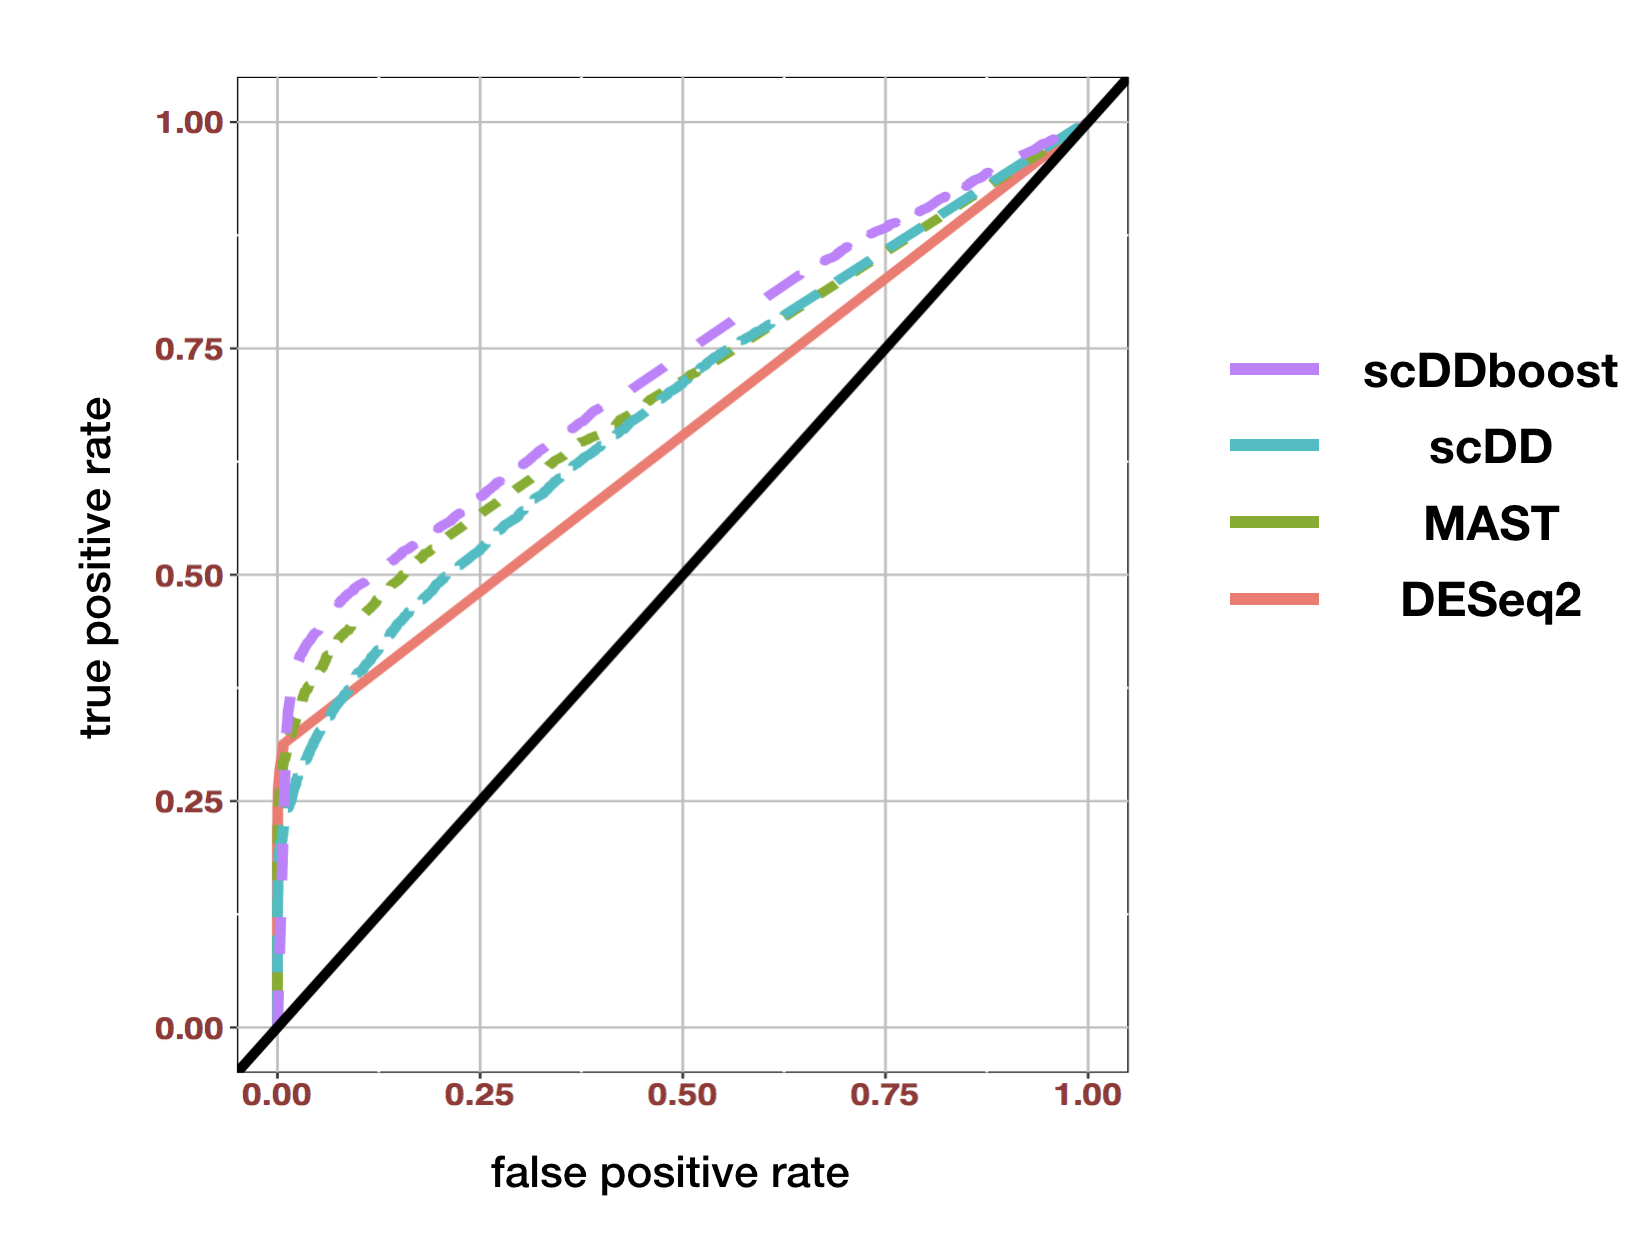
\includegraphics[width = 0.4\textwidth]{roc.png}
  \caption{Roc curve of scDDboost, scDD, MAST and DESeq2, scDDboost has largest area under the roc curve. Roc curves of other three methods are similar. For those roc curve there is bigger difference at low level of false positive rate, as scDDboost identified twice many true DD genes as other methods.}
  \label{fig:5}
\end{figure}

Since we are modeling gene transcript within each subtype as negative binomial distributed and we only test one parameter(mean) change among subtypes. In some scenario, it could be insufficient to model the variability within subtype. Even though there is no mean expression change among subtypes but more subtle distributional change occurred among subtypes changed, EBSeq would fail to detect the discrepancies between subtypes, thus limit power of scDDboost.\\
\newpage
\section{Examples}
\subsection{real data}
We use ten datasets from conquer\cite{ref:Cq} to test performance of our method on real data. We compare our results with scDD\cite{ref:scDD}, MAST\cite{ref:MAST} and DESeq2\cite{ref:Des}\\
\begin{table}[ht]
\centering
\begin{tabular}{ |p{3cm}|p{6cm}|p{2cm}|p{1cm}|p{1cm}|}
\hline
 Data set & Compared cell subsets & Number of cells/condition & Organism & Ref\\
 \hline
 \hline
 GSE45719 & 16-cell stage blastomere vs Mid blastocyst cell (92-94h post- fertilization) & 50, 60 & mouse & \cite{Deng193}\\
 \hline
 GSE45719null &  16-cell stage blastomere & 50 & mouse &  \cite{Deng193}\\
 \hline
 GSE48968-GPL13112 & BMDC (1h LPS stimulation) vs BMDC(4h LPS stimulation) & 96, 95 & mouse & \cite{Shalek}\\
 \hline
 GSE48968-GPL13112null & BMDC (1h LPS stimulation) & 96 & mouse & \cite{Shalek}\\
 \hline
 GSE60749-GPL13112 & v6.5 mouse embryonic stem cells, culture conditions: 2i+LIF vs v6.5 mouse embryonic stem cells, culture conditions: serum+LIF & 90, 94 & mouse & \cite{Kumar}\\
 \hline
 GSE60749-GPL13112null & v6.5 mouse embryonic stem cells, culture conditions: 2i+LIF & 90 & mouse & \cite{Kumar}\\
 \hline
 GSE74596 & NKT0 vs NKT17 & 45,44 & mouse & \cite{Engel}\\
 \hline
 GSE74596null & NKT0 & 45 & mouse & \cite{Engel}\\
 \hline
 EMTAB2805 & G1 vs G2M & 96,96 & mouse & \cite{EMTAB}\\
 \hline
 EMTAB2805null & G1 & 96 & mouse & \cite{EMTAB}\\
 \hline
 GSE63818-GPL16791 & Primordial Germ Cells, develop- mental stage: 7 week gestation vs Somatic Cells, developmental stage: 7 week gestation & 39,26 & mouse & \cite{Guo}\\
 \hline
 GSE71585-GPL13112 & Chrna2 tdTpositive vs Cux2 tdTpositive & 84, 124 & mouse & \cite{Tasic}\\
 \hline
GSE71585-GPL13112null & Chrna2 tdTpositive & 84 & mouse & \cite{Tasic}\\
\hline
GSE75748 & NPC vs DEC & 64, 87 & human & \cite{chu}\\
\hline
GSE75748 & NPC & 64 & human & \cite{chu}\\
\hline
GSE75748 & DEC vs EC & 70, 64 & human & \cite{chu}\\
\hline
GSE75748 & DEC & 70 & human & \cite{chu}\\
\hline
GSE64016null & H1 exp1 vs H1 exp2 & 64, 87 & human & \cite{oscope}\\
\hline
\end{tabular}
\captionof{table}{single cell transcripts profiles used for differential expression or distribution method evaluation}
\end{table}
\hfill\\
We have table of numbers of differentially expressed genes of each dataset by MAST and DESeq2, and numbers of differentially distributed genes of each dataset by scDDboost and scDD.\\

\begin{table}[ht]
\centering
\begin{tabular}{ |p{2cm}|p{2cm}|p{2cm}|p{2cm}|p{2cm}|p{2cm}|p{2cm}|}
\hline
Data set & scDDboost & scDDboost-sc3 & scDD & MAST & DESeq2 & total number of genes\\
\hline
\hline
GSE45719 & 5758 & 4228 & 6416 &5652 & 11202 & 45686\\
\hline
GSE48969-GPL13112 & 11691 & 9819 & 2080 & 3396 & 9542 & 45686\\
\hline
GSE60749-GPL13112 & 19215 & 19168 &  18074 & 13674 & 23178 & 45686\\
\hline
GSE74596 & 2301 & 1355 & 1409 & 540 & 3796 & 45686\\
\hline
EMTAB 2805 & 5295 & 3748 & 2202 & 1088 & 5391 & 45686\\
\hline
GSE63818-GPL16791 & 3948 & 3480 & 1365 & 873 & 8934 & 45686\\
\hline
GSE71585- GPL13112 & 2902 & 1460 & 1622 & 2572 & 7378 & 24057 \\
\hline
NPC-DEC & 4377 & 3211 & 5982 & 6666 & 8439 & 19037\\
\hline
DEC-EC & 3402 & 3023 & 3818 & 5429 & 8127 & 19037\\
\hline
H1 exp1-H1 exp2 &  0 & 0 & 1300 & 2077 & 2841 & 16579\\
\hline
\end{tabular}
\captionof{table}{number of DD genes detected by different methods}
\end{table}

We found that bulk method DESeq2 tends to have the most number of DE genes. But among single cell methods, scDDboost usually identified the most DD genes. Further we observed quite a few genes uniquely identified by scDDboost are likely to have different distribution across conditions. For example, figure 5, we use violin plot to demonstrate the log expression profiles among DEC and EC. \\
\begin{figure}[H]
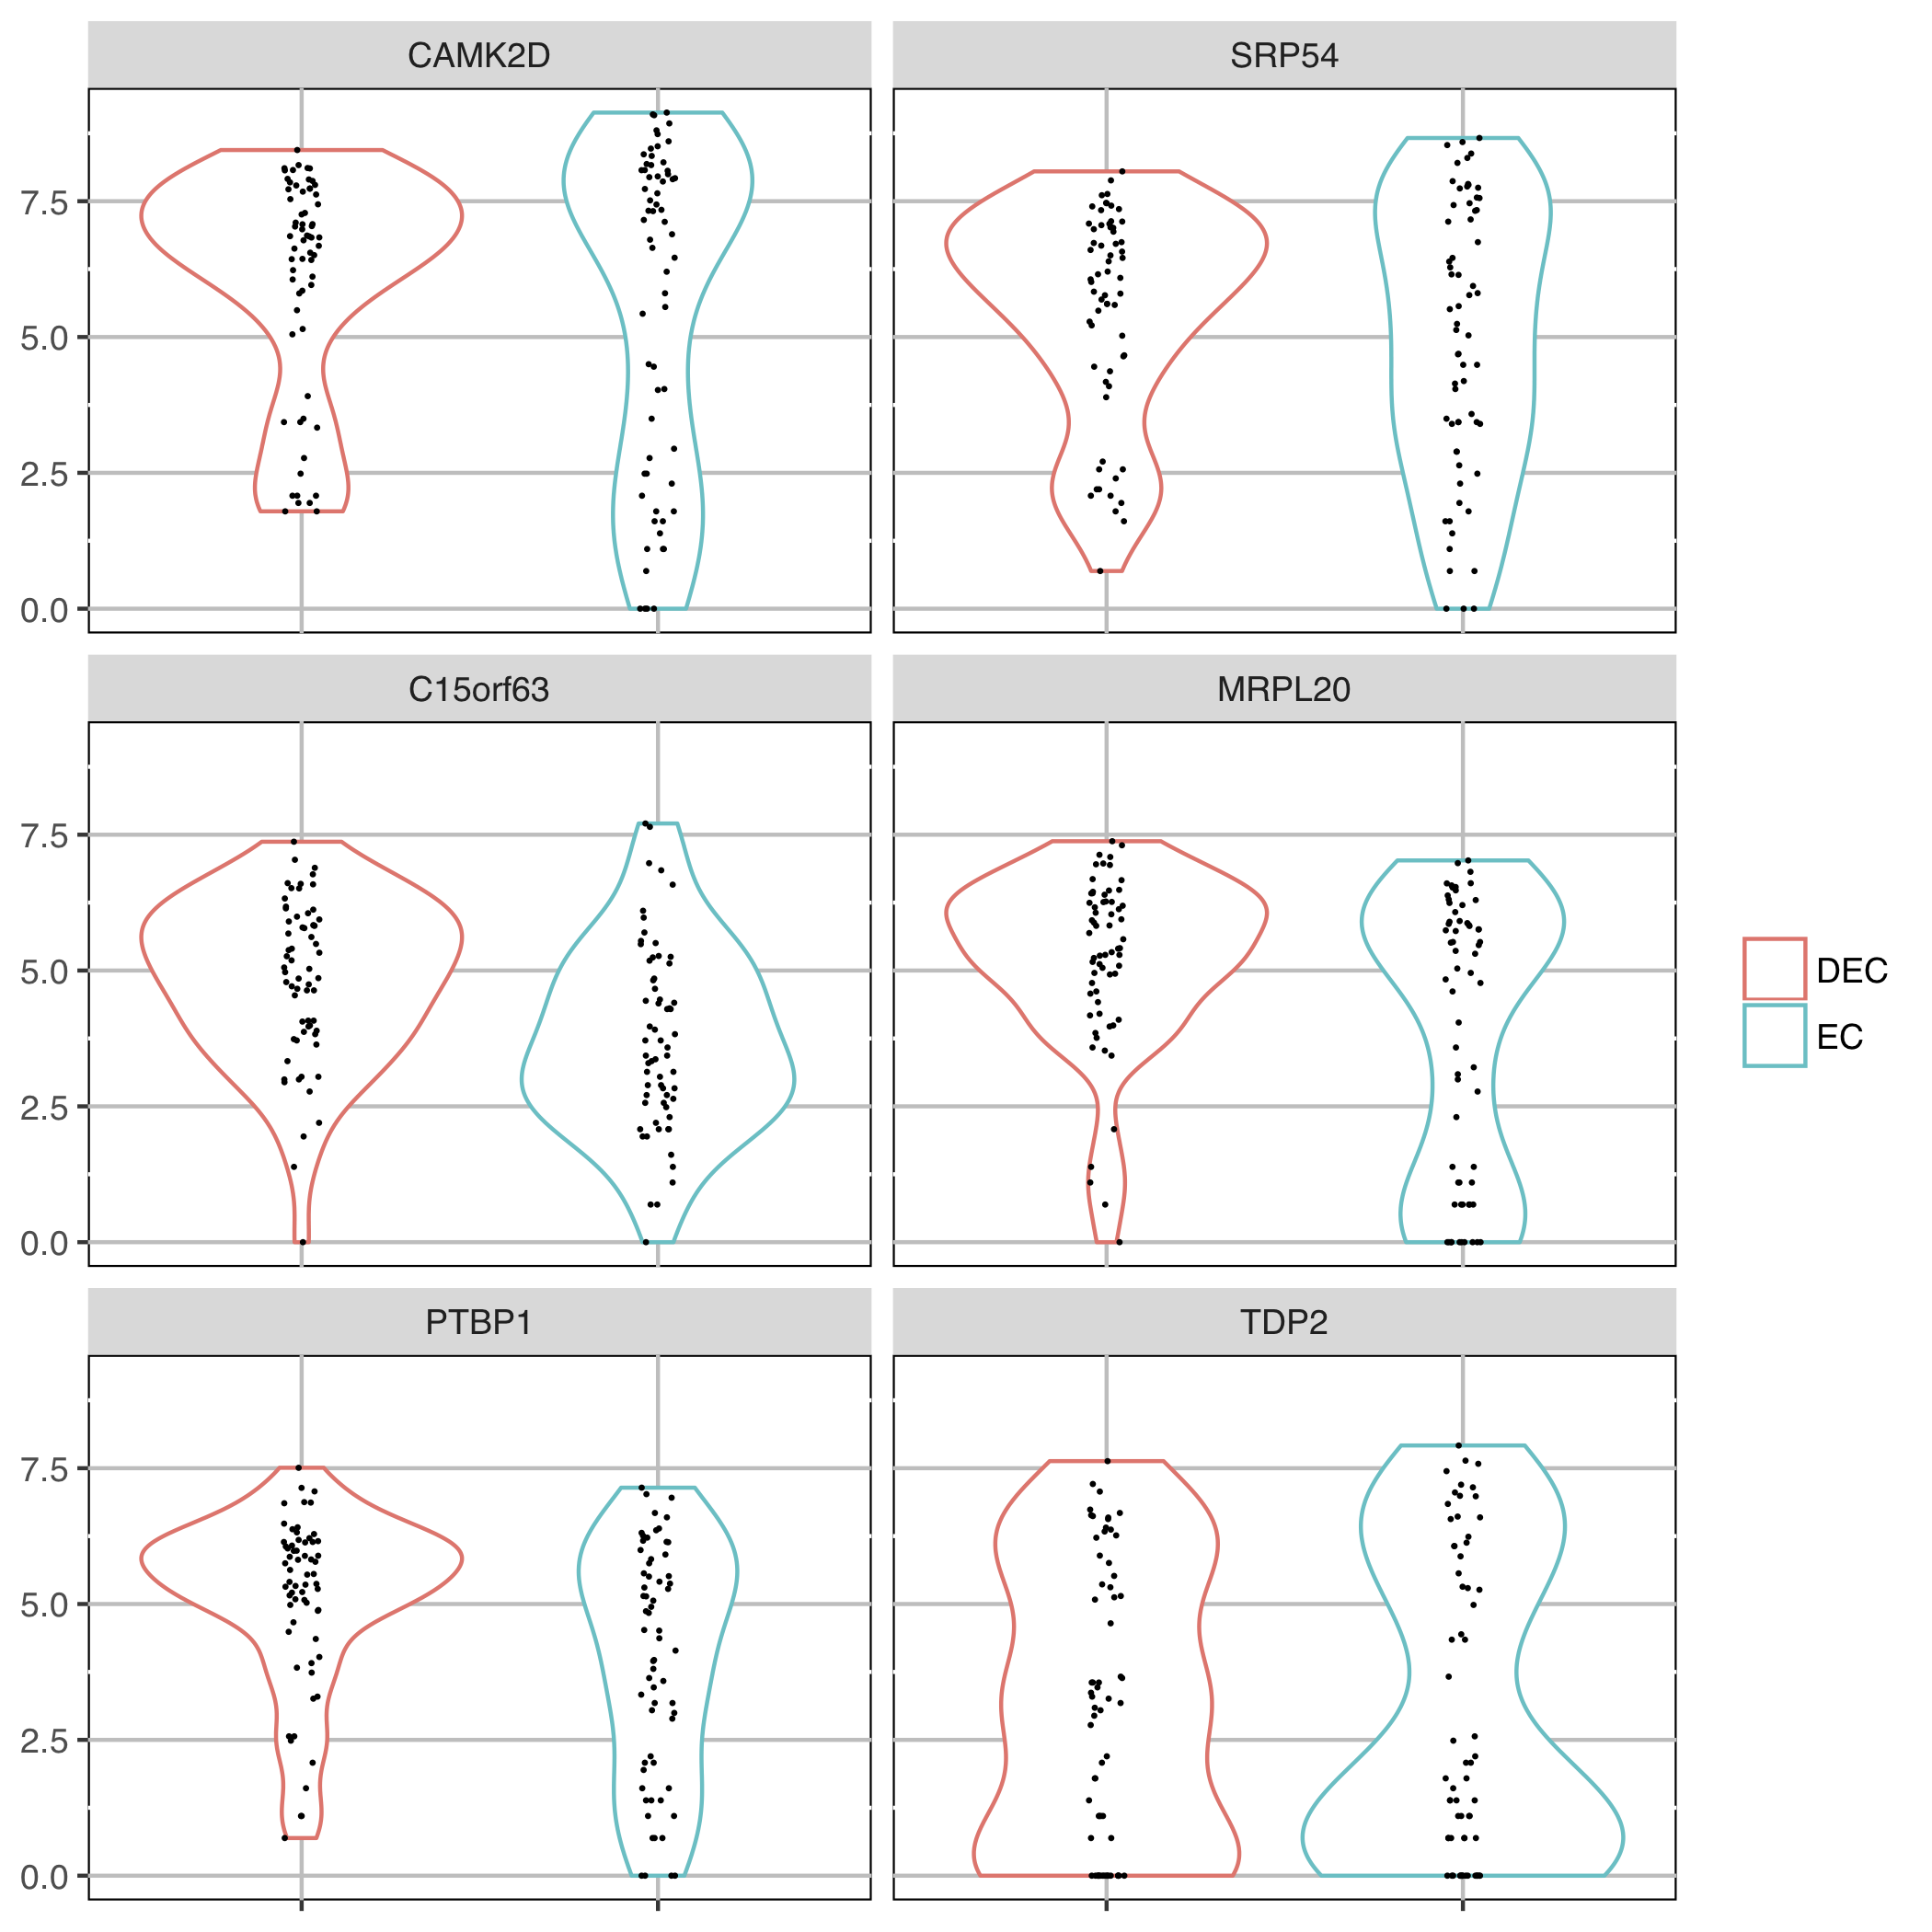
\includegraphics[width = 0.6\textwidth]{density_DEC_dd.png}
 \caption{ Densities of log transformed transcripts, 6 DD genes uniquely identified by scDDboost, for data GSE75748, DEC vs. EC, We observe some of the genes are different distributed across conditions.}
  \label{fig:6}
\end{figure}

\subsection{FDR}
Although bulk methods seems to be the most powerful one, we found it also has a higher false discovery rate comparing to single cell methods. We validate false discovery rate on ten null datasets from table 1. For each null dataset, we randomly split the cells from one condition into two subsets and test difference of gene expression between those subsets. Since the two subsets of cells actually came from same condition, there should not be any differential distributed genes, any positive call would be a false positive. We repeat the random split and testing for five times on each null data set. We evaluate the type I error control for the methods returning nominal p-values, by recording the fraction of genes(with a valid p-value) that are assigned a nomial p-value below 0.05 (figure 5).\\
scDDboost could control FDR since we assume cells are sampled from population composed of different subtypes. Cells from one subtype are equal likely to be assigned to either one of the two subsets. Consequently, it is very likely that proportions of subtypes remain unchanged among the two subsets.

\begin{figure}[H]
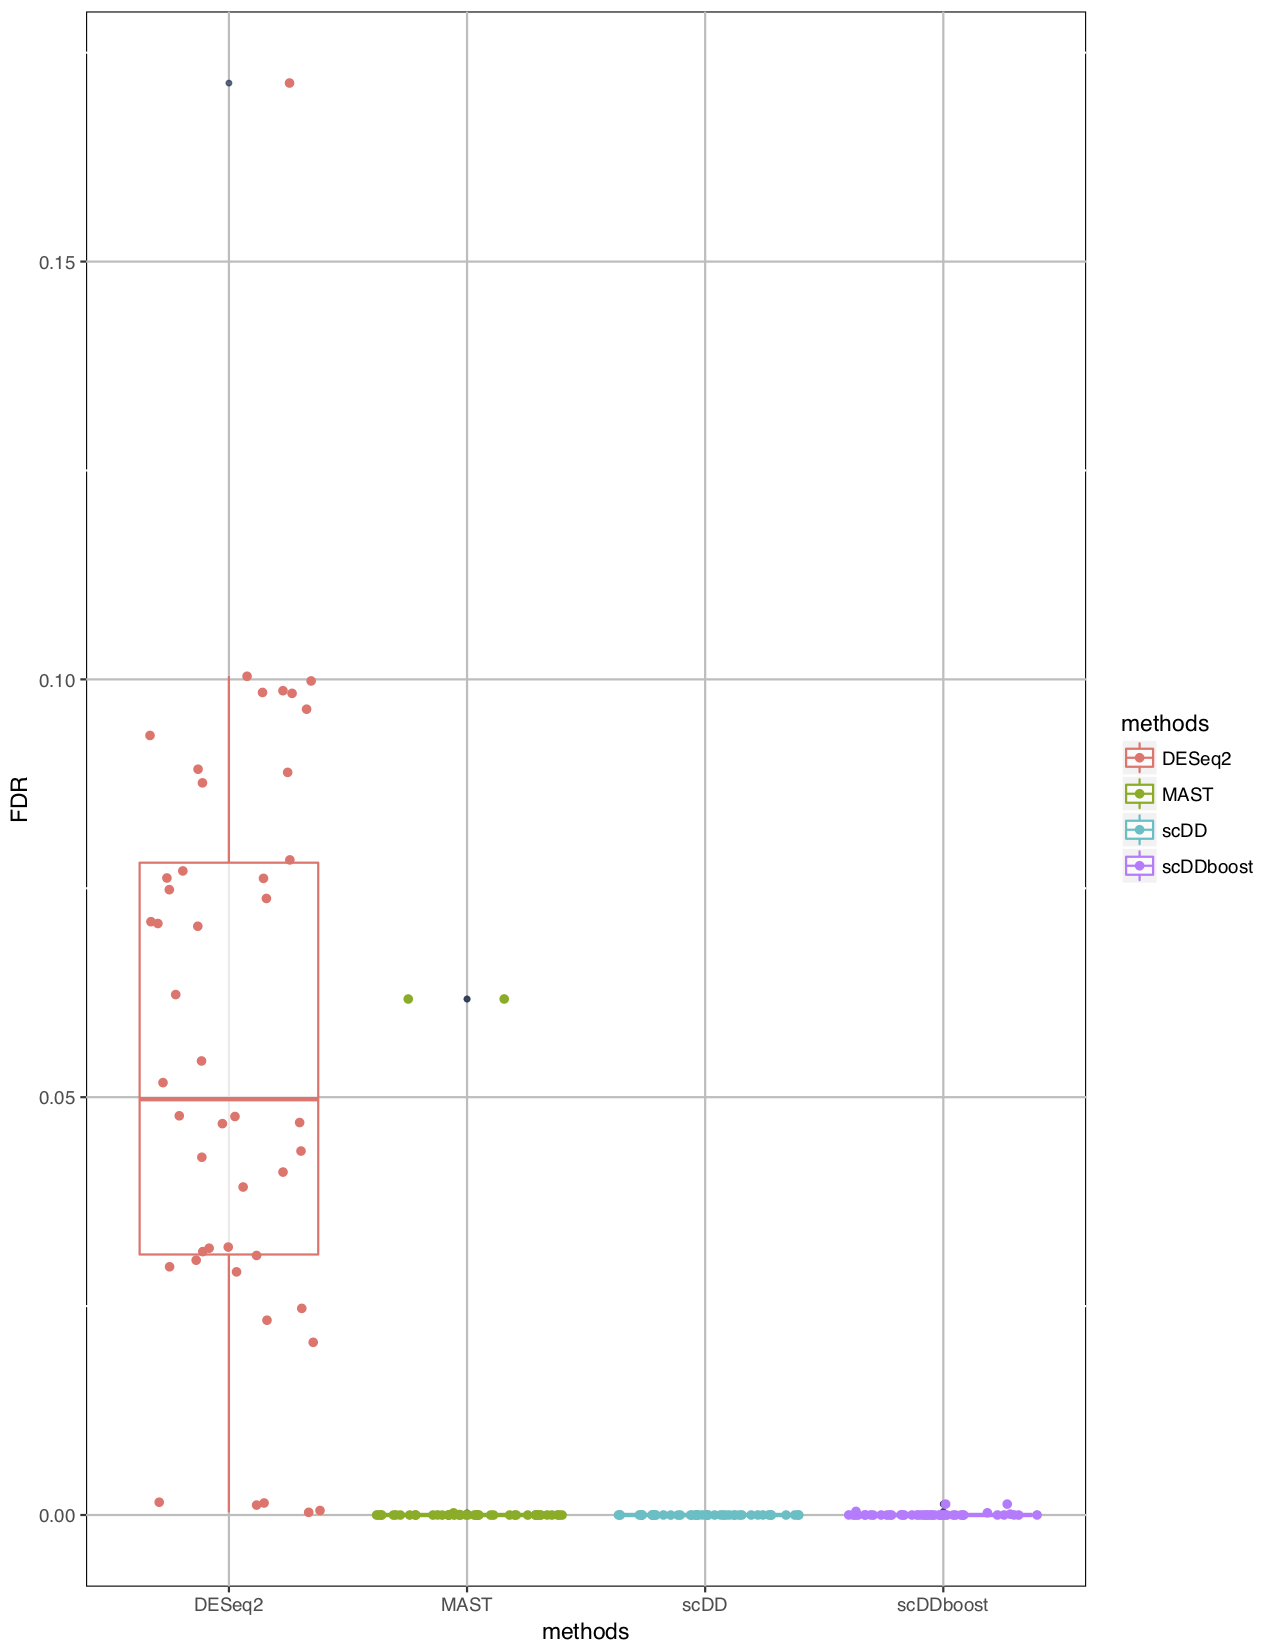
\includegraphics[width = 0.4\textwidth]{FDR.png}
 \caption{FDR of scDDboost, scDD, MAST and DESeq2 on null dataset from table 1, DESeq2 usually identify a lot but may lose the control of type I error. While other single cell methods could control FDR. ***This procedure for testing FDR,  we randomly split a population into two samples, so it is highly likely proportion of subtypes remain same among these two samples, scDDboost always give small PDD and almost make no false positive call. This is kind different from really examining the FDR of scDDboost, where we have different proportions across conditions, but we do not want false call on those genes without mean expression change even there is proportion change. In this case, it actually reduce to the FDR of EBSeq whether we make correct posterior inference on DE pattern. The test of proportion is only done once, so scDDboost could still control FDR*** }
  \label{fig:7}
\end{figure}

\subsection{number of subtypes}
From our empirical experience, it is typical $K$ will not be larger than 8. We demonstrate the change of posterior probabilities of differential distribution given different number of subtypes at data GSE75748 and GSE48968. In both cases, if allowing one more subtype would result in a lot increases in posterior probabilities, which suggests that the number of subtypes is underestimated since we found more distribution differences between conditions given one more mixture component. If posterior inference is stable after increasing the number of subtypes, then we consider previous number of subtypes to be optimal. 
\begin{figure}[H]
\minipage{0.5\textwidth}
  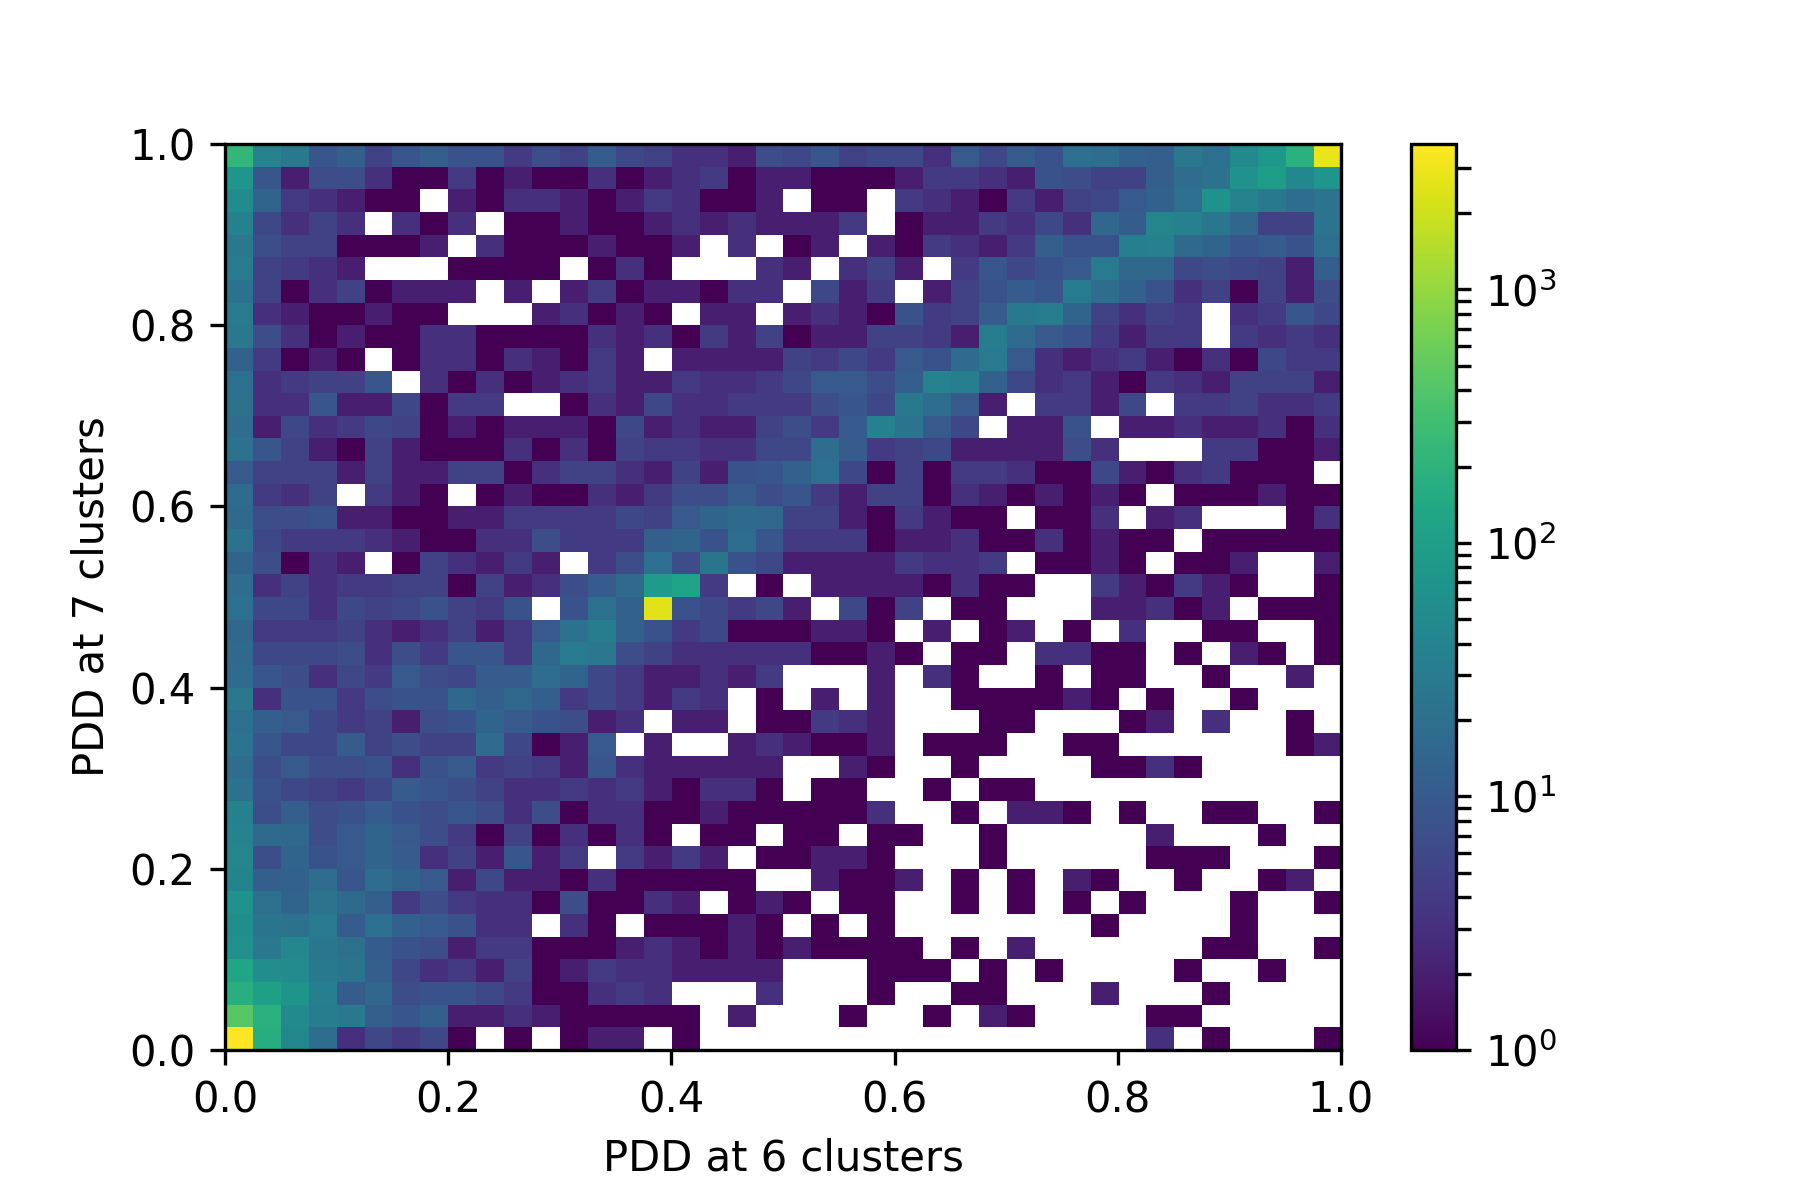
\includegraphics[height = 5cm, width=\linewidth]{DN_67.png}
\endminipage\hfill
\minipage{0.5\textwidth}
  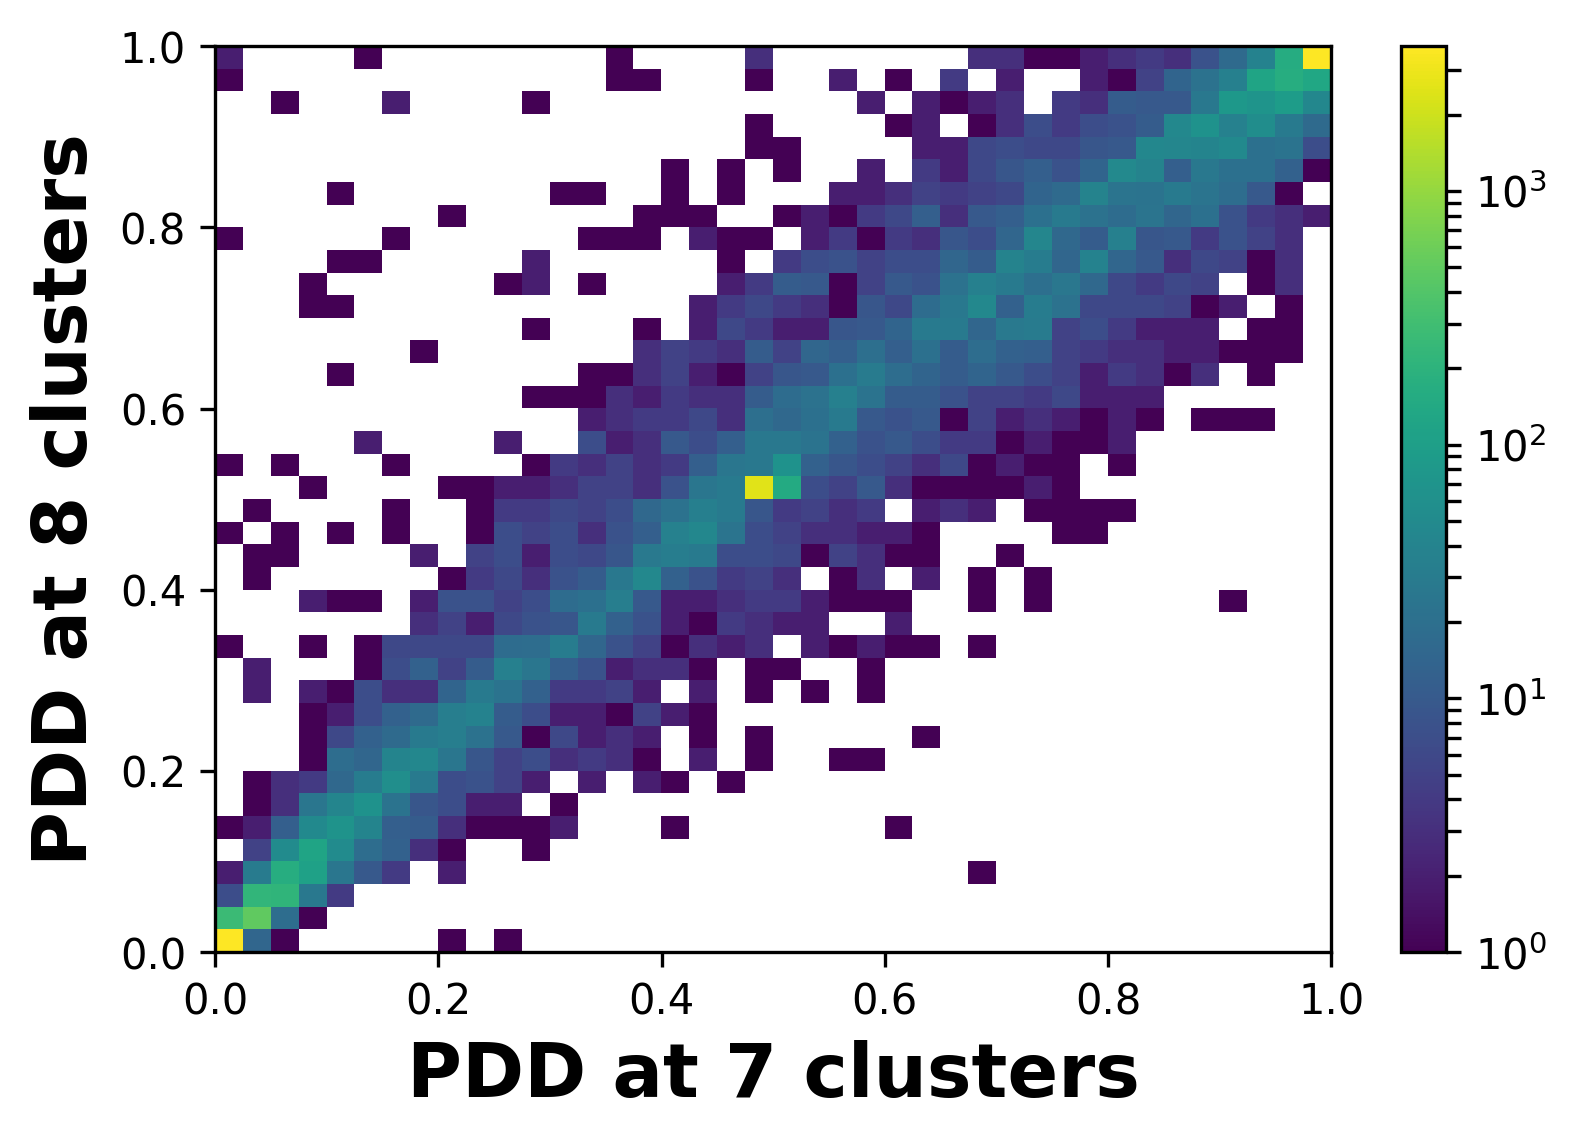
\includegraphics[height = 5cm, width=\linewidth]{DN_78.png}
\endminipage\hfill
\caption{selecting number of subtypes for data GSE75748, we observe posterior probabilities become stable at more than 6 subtypes. Since increasing number of subtypes tends to decrease sample size of each subtypes, make complicate constraints for equivalent distribution and inflate estimated PDD.  We select number of subtypes to be 7}
\end{figure}
\begin{figure}[H]
\minipage{0.5\textwidth}
  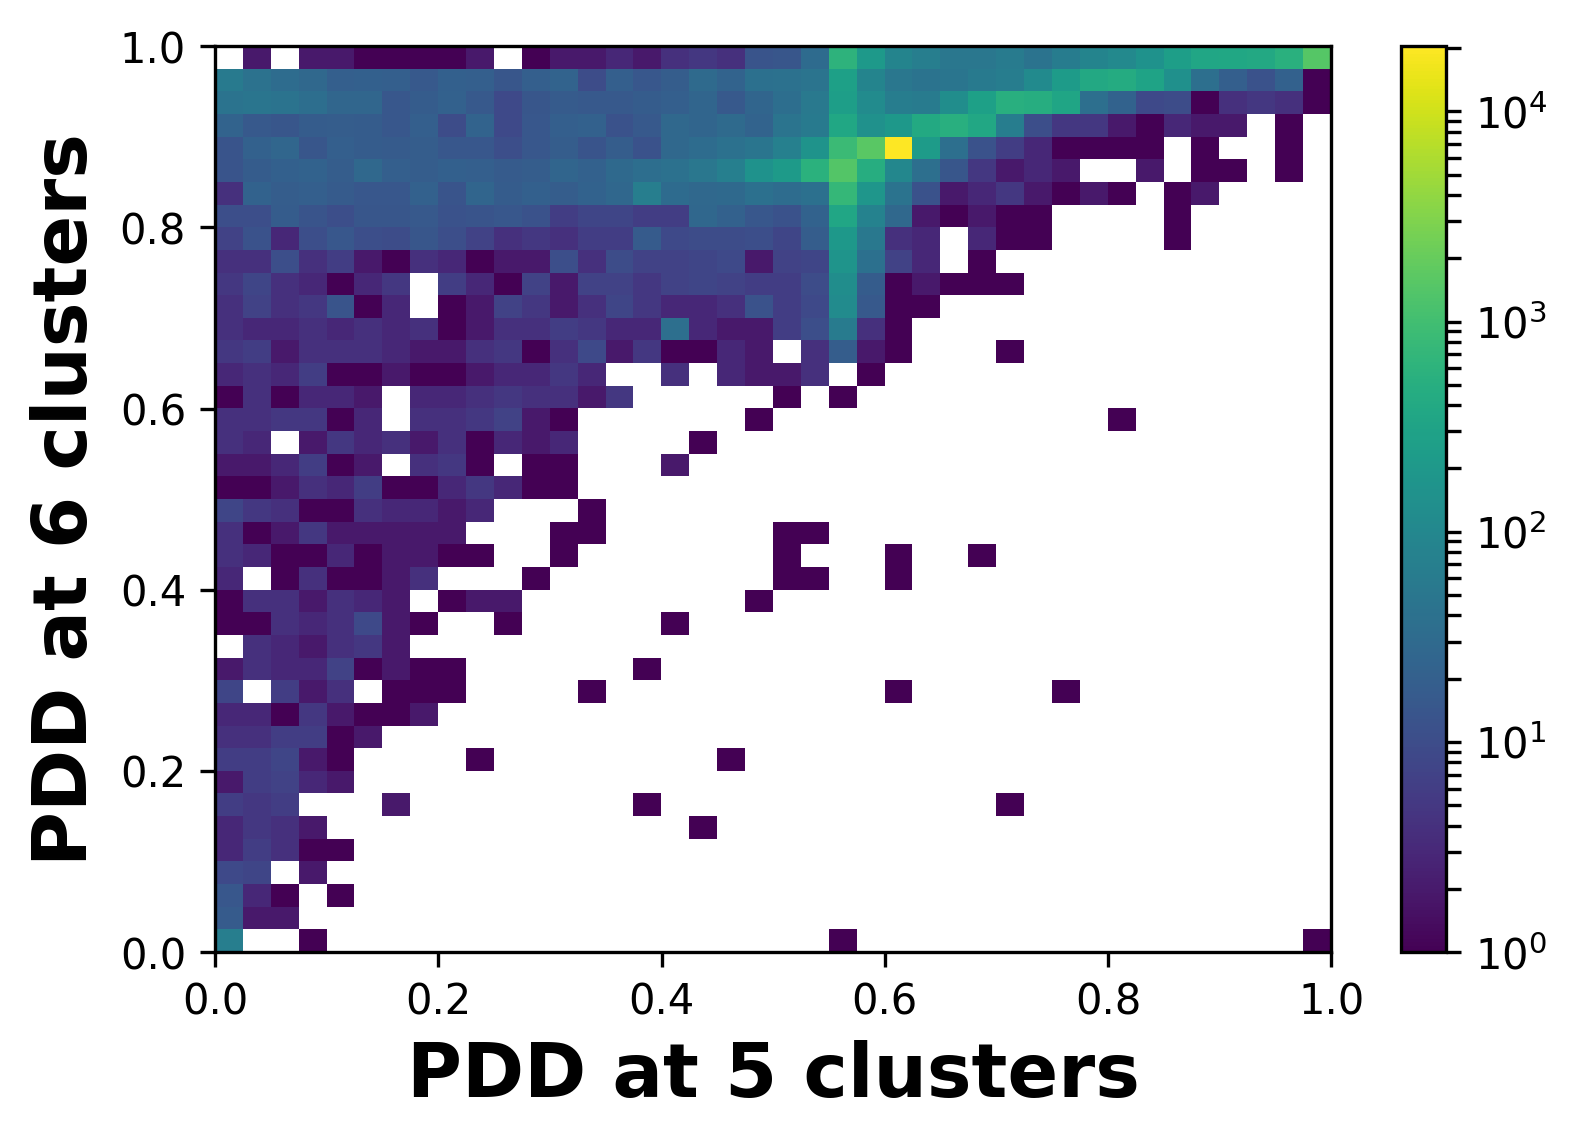
\includegraphics[height = 5cm, width=\linewidth]{G48_56.png}
\endminipage\hfill
\minipage{0.5\textwidth}
  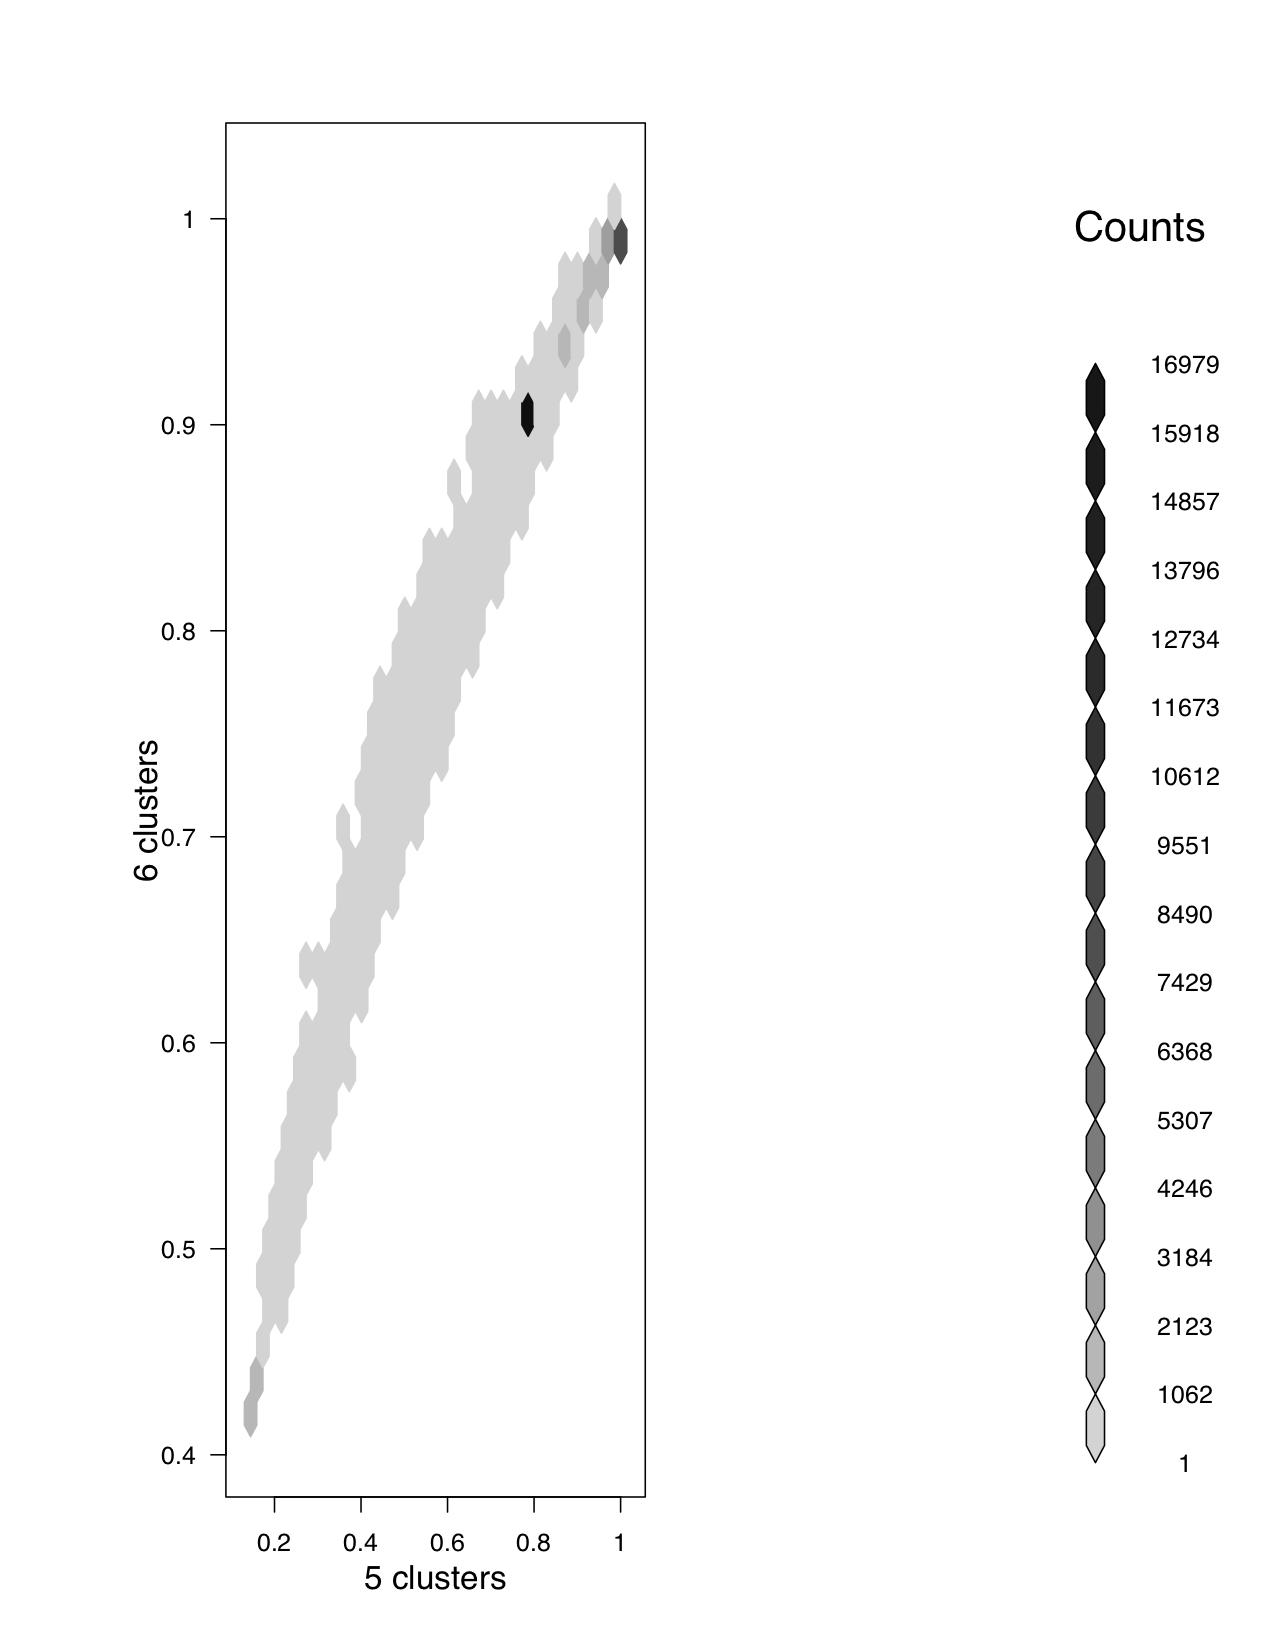
\includegraphics[height = 5cm, width=\linewidth]{G48_67.png}
\endminipage\hfill
\caption{selecting number of subtypes for data GSE48968, we observe posterior probabilities become stable at more than 5 subtypes}
\end{figure}

\subsection{bursting parameters}
D3E\cite{ref:d3e} is a distributional method that can identify bursting parameters of transcripts. Rate of promoter activation, rate of promoter inactivation and the rate of transcription when the promoter is in the active state are estimated by D3E.  We investigate DD genes identified by scDDboost and their change of those three parameters on dataset EMTAB2805\\

\begin{figure}[H]
\vspace{-\parskip}
\minipage{0.33\textwidth}
  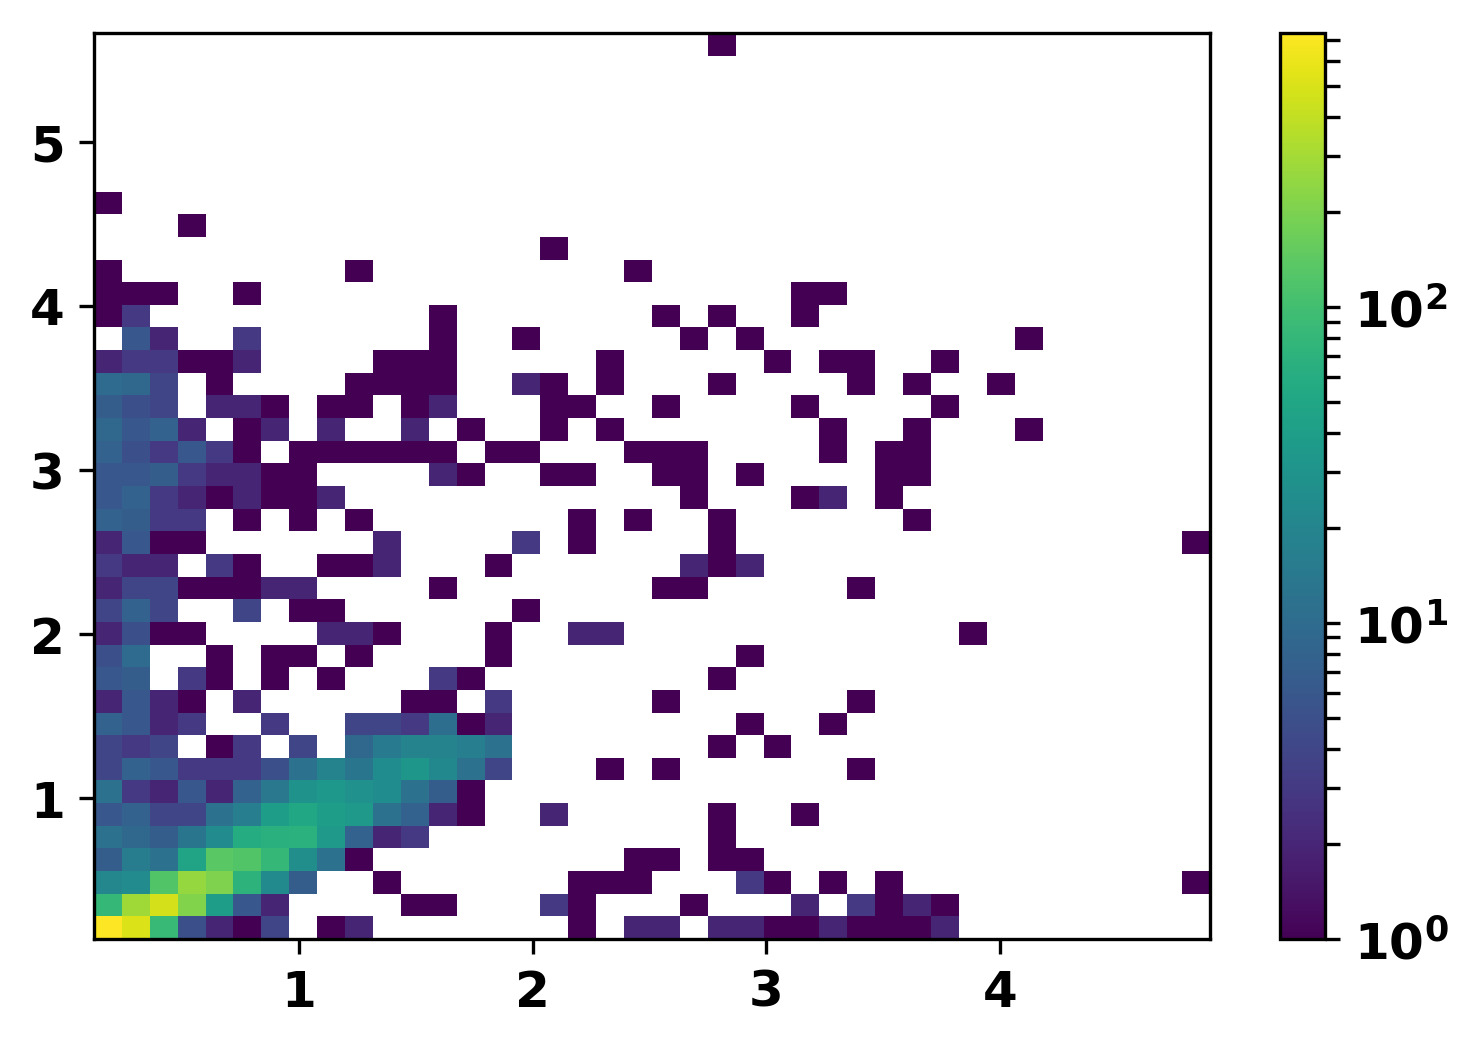
\includegraphics[clip,width=\textwidth]{act.png}
\endminipage
\minipage{0.33\textwidth}
  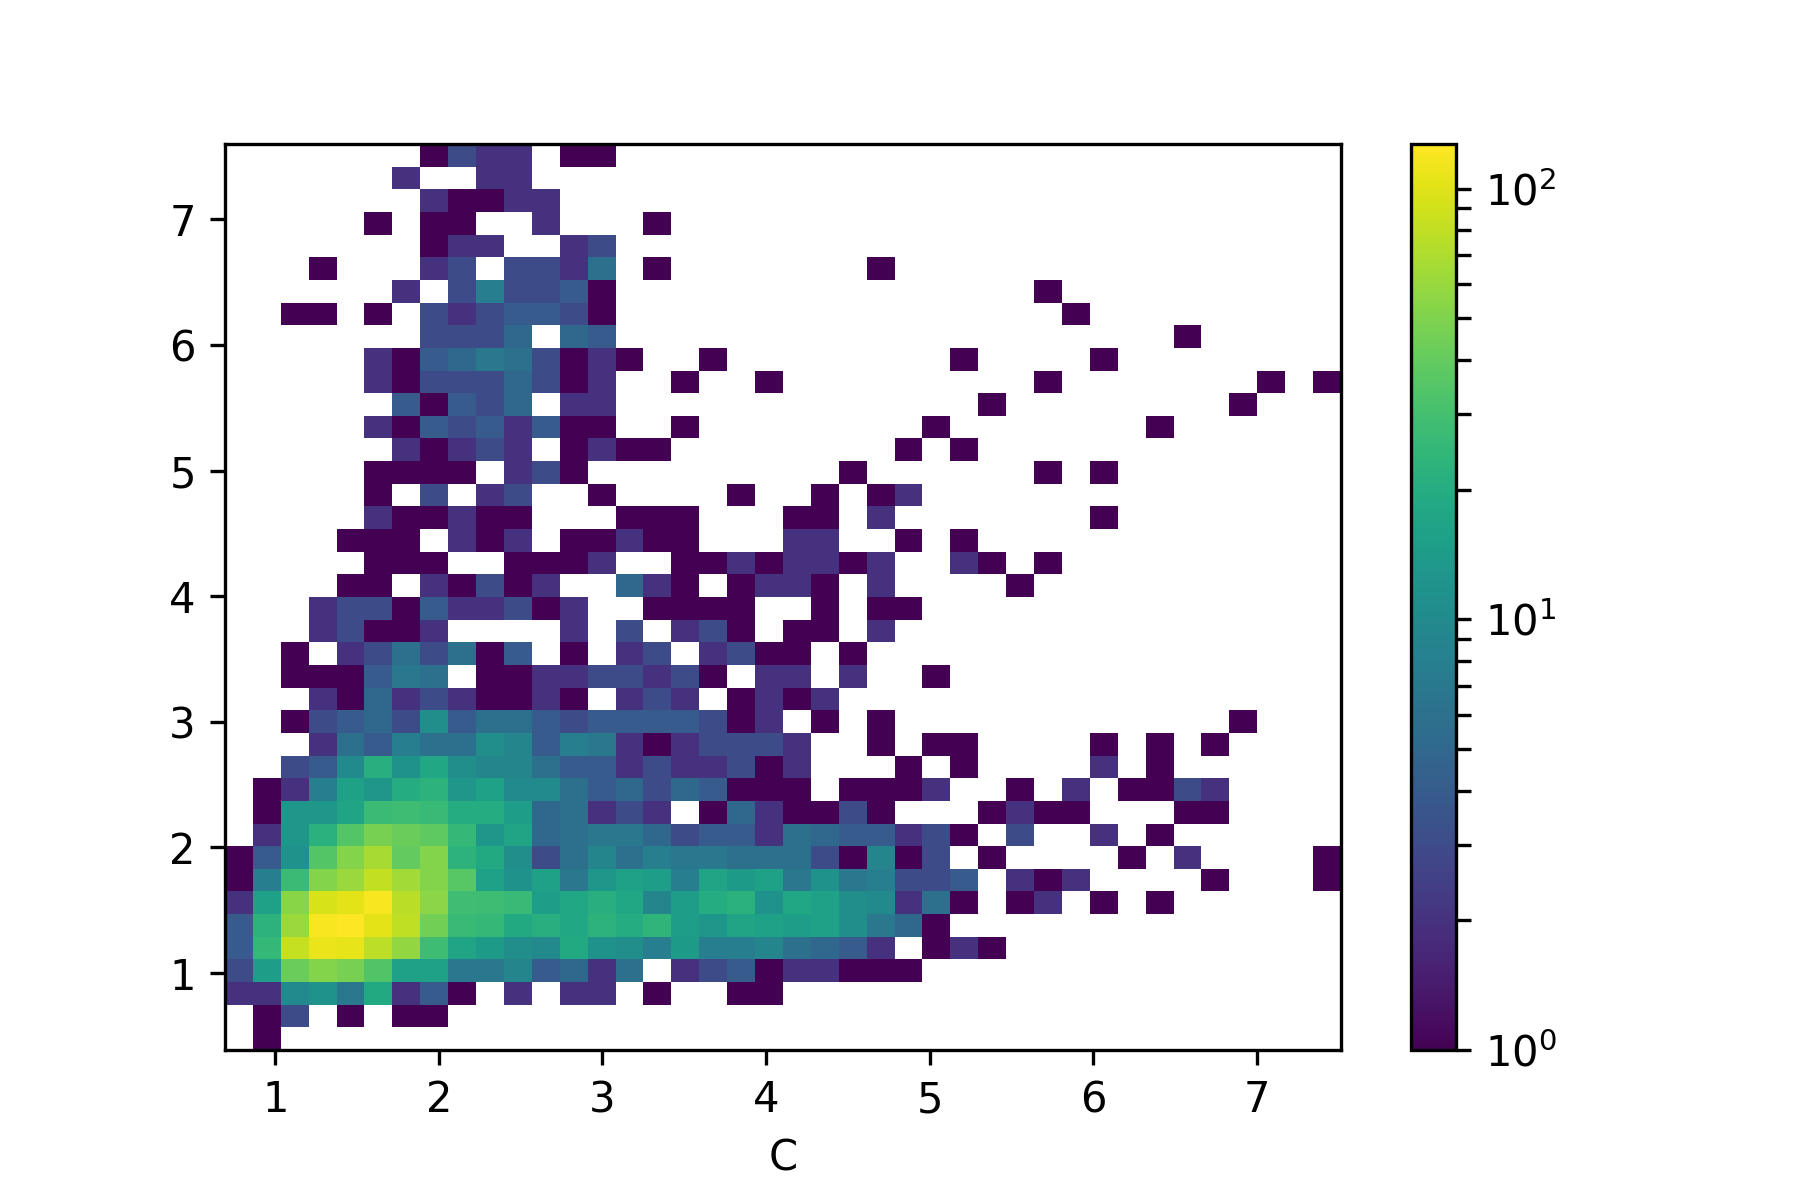
\includegraphics[clip,width=\textwidth]{in_act.png}
  \endminipage
 \minipage{0.33\textwidth}
  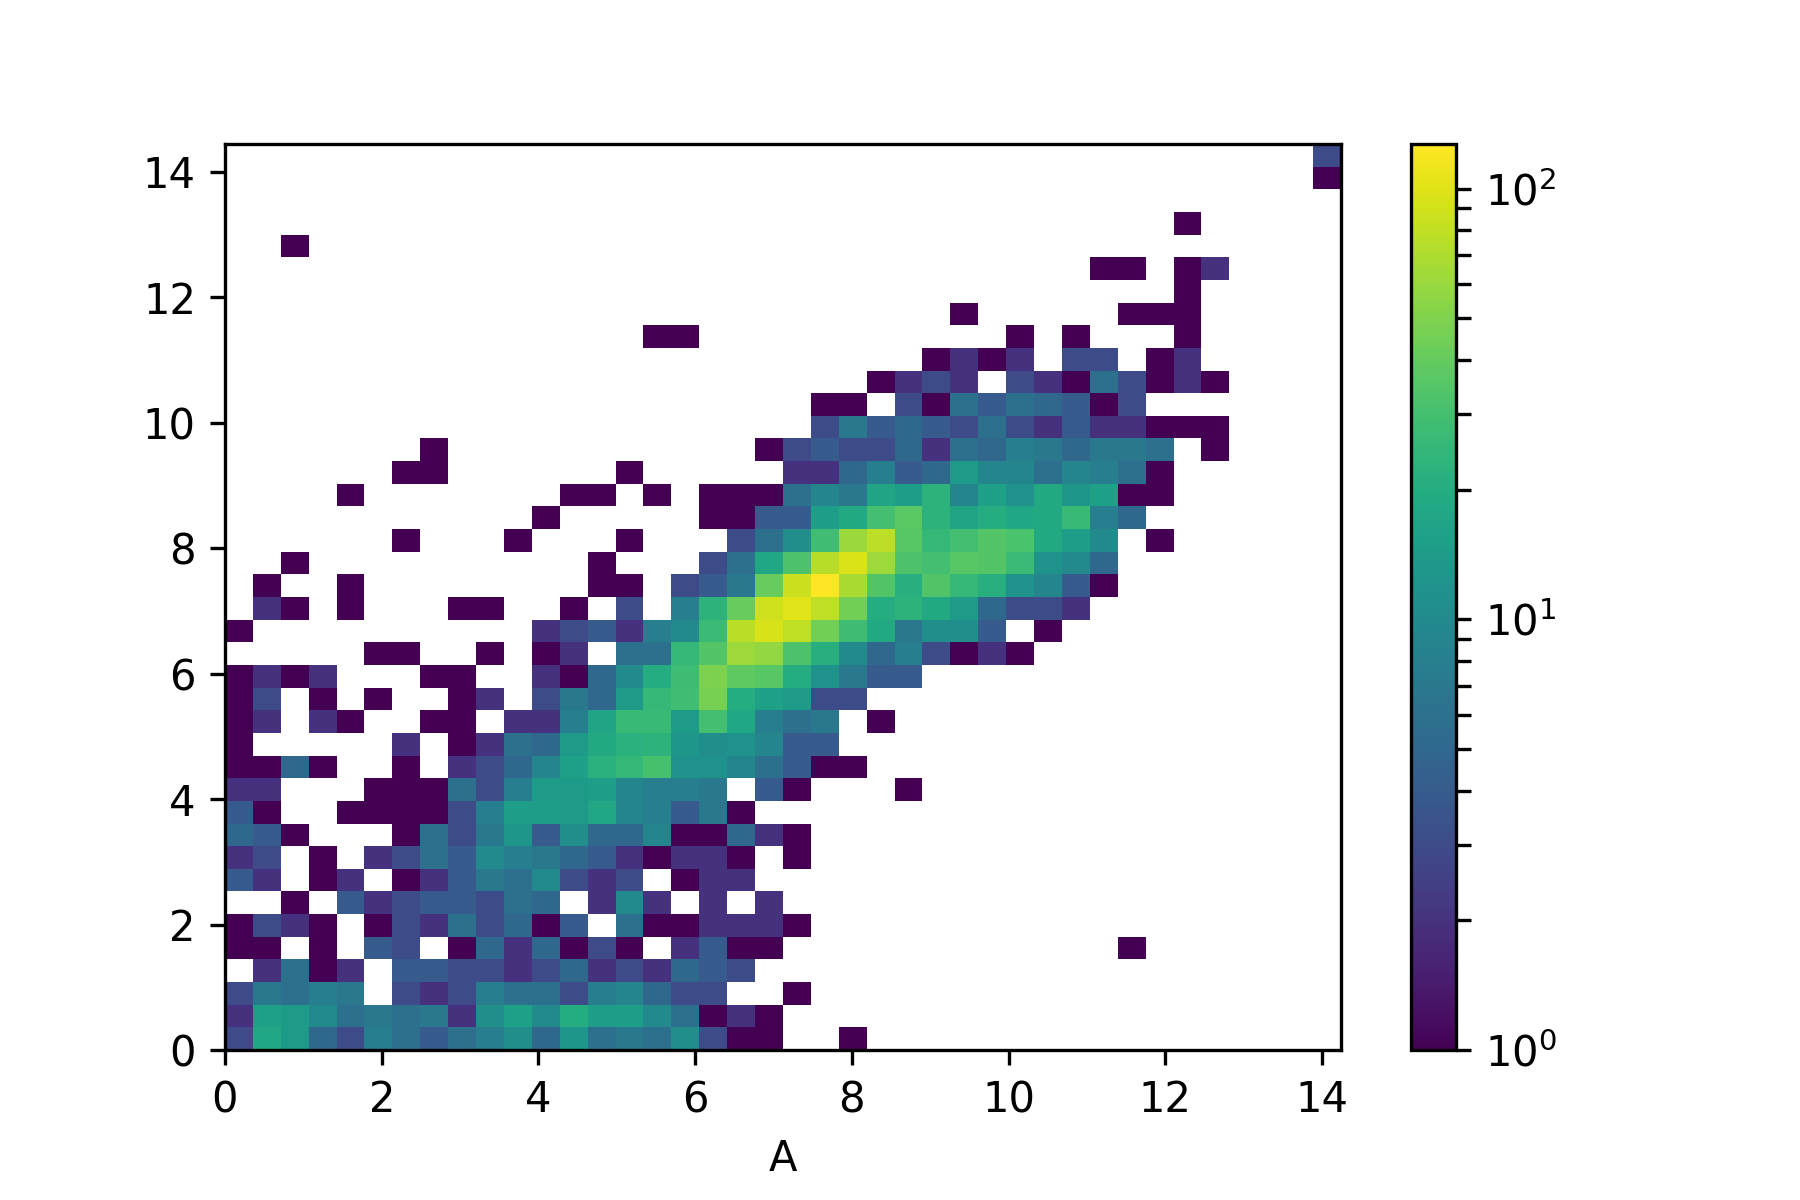
\includegraphics[clip,width=\textwidth]{t_rate.png}
  \endminipage
\captionof{figure}{2D histogram for bursting parameters of DD genes identified by scDDboost from dataset EMTAB2805 estimated by D3E. Left panel  : comparison of rate of promoter activation between two conditions, similarly, middle panel  : rate of promoter inactivation and right panel: rate of transcription when the promoter is in the active state. We observe that difference between transcription rate is smaller compare to difference between the activation and inactivation rate. ***other methods also observe similar phenomena, this is not unique to scDDboost, main reason is that estimation from D3E tends to give larger difference in activation and inactivation rate than transcription rate. We may argue the major factor to drive DD genes are activation and inactivation rate (proportions of different subtyps), so it make sense to consider mixture model like scDDboost.***}
\end{figure}
We observed that DD genes identified by scDDboost tends to have similar transcription rate when the promoter is active across condition, while there are lots of variabilities in the action and inactivation rate. These results reveal that DD genes identified by scDDboost are driven by the change of activation and inactivation rates. 



\section{asymptotic properties}\hfill\\

To investigate asymptotic properties we first give the expression of posterior probability. Since there is no information favorable of any particular $A_\pi$, we select discrete uniform distribution as the prior for it, then the posterior probability is
\begin{align}
p(A_\pi | t^1, t^2) = c*\sum_{\pi' \text{ refines } \pi} p(t^1 | t^1_{\pi'})\, p(t^2 |  t^2_{\pi'} )
 \, p( t^1_{\pi'}, t^2_{\pi'} | A_{\pi'} )
\end{align}
for a normalizing constant $\frac{1}{c} = \underset{\pi' \in \Pi}\sum p(t^1 | t^1_{\pi'})\, p(t^2|  t^2_{\pi'} )
 \, p( t^1_{\pi'}, t^2_{\pi'} | A_{\pi'} )$.
 
Let $\Omega = \{(\phi, \psi): \overset{K}{\underset{i = 1}\sum}\phi_i = \overset{K}{\underset{i = 1}\sum}\psi_i = 1, \phi_i \geq 0, \psi_i \geq 0 , i = 1,..., K\}$ be the whole space. There is a subset of $\Omega$ we lack posterior inference. Let us first see an example:
\begin{figure}[h]
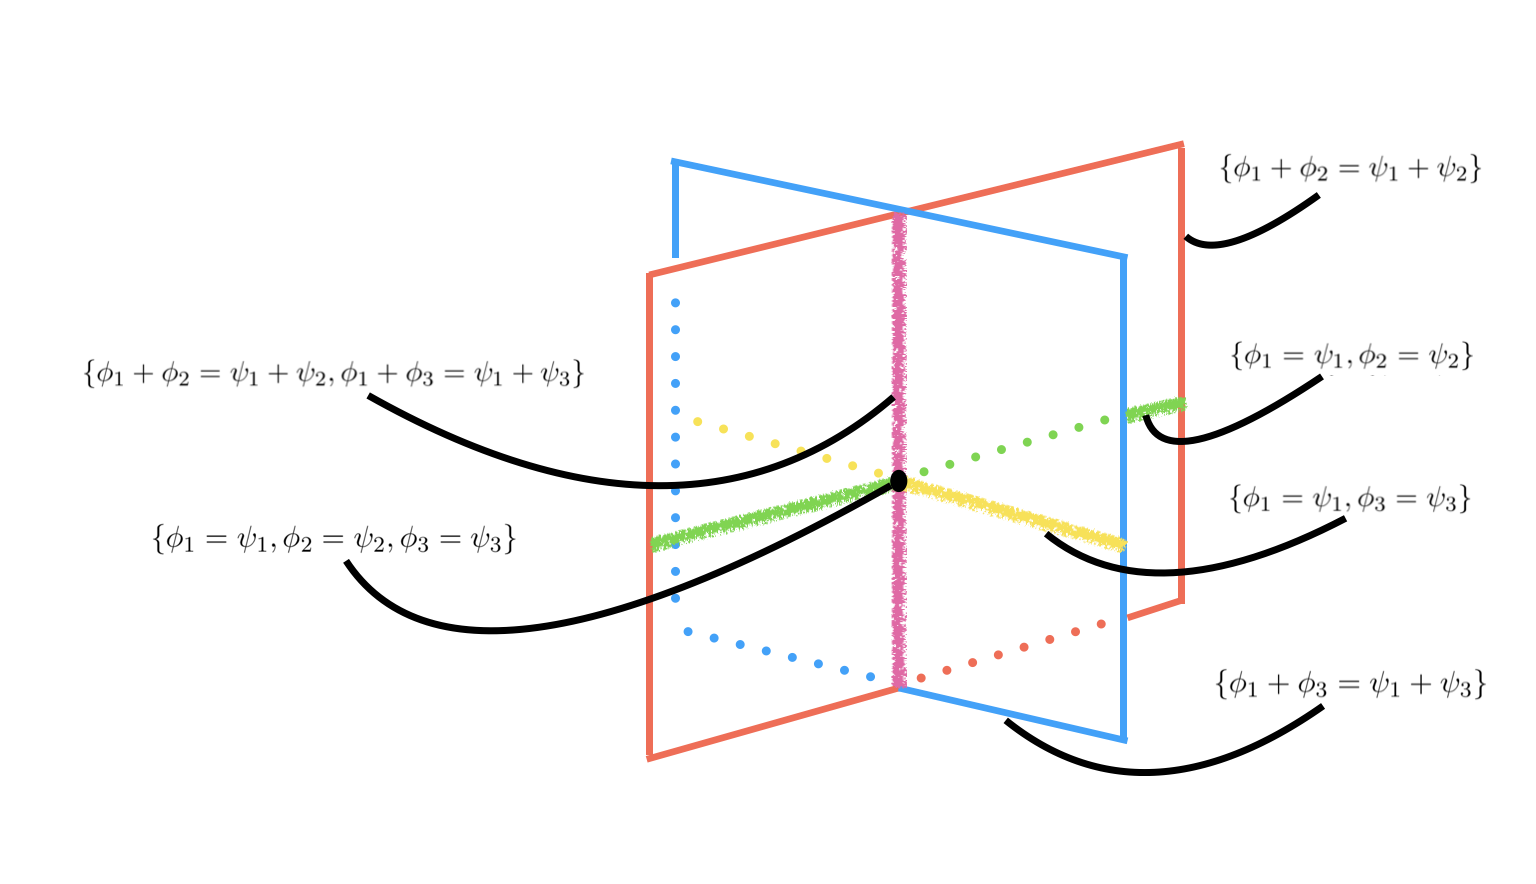
\includegraphics[scale = 0.5]{overlap.png}
 \caption{Four subtypes of cells,  simplexes of $(\phi,\psi)$ satisfying different constraints.}
  \label{fig:1}
\end{figure}
\hfill\\
In figure 11, there are four subtypes, the rectangle with magenta boundary is a simplex $A_{\pi_1} = \{(\phi,\psi) : \phi_1 + \phi_2 = \psi_1 + \psi_2\}$, the rectangle with blue boundary is a simplex $A_{\pi_2} = \{(\phi,\psi) : \phi_1 + \phi_3 = \psi_1 + \psi_3\}$. The green line refers to $A_{\pi_3} = \{(\phi,\psi) : \phi_1 = \psi_1, \phi_2 = \psi_2\}$, the yellow line refers to $A_{\pi_4} = \{(\phi,\psi) : \phi_1 = \psi_1, \phi_3 = \psi_3\}$, the purple line refers to $A_{\pi_5} = \{(\phi,\psi) : \phi_1 + \phi_2 = \psi_1 + \psi_2, \phi_1 + \phi_3 = \psi_1 + \psi_3\}$, which is the intersection of $A_{\pi_1}$ and $A_{\pi_2}$, and finally the black dot which is the intersection of those three lines refers to the simplex with finest partitions, $\phi_i = \psi_i, \forall i = 1,..,4$. We lack posterior inference for $(\phi,\psi)$ along the purple line except the black dot. While on the green line, yellow line and black dot, we have consistent posterior inference(theorem 2). To explain why some space lacking posterior inference and define such space, we define a special subset $A_\pi^*$ of simplex $A_\pi$. $A_\pi^* = A_\pi\setminus \underset{\tilde{\pi} \text{ is not coarser than } \pi }\cup A_{\tilde{\pi}}$, $A_\pi^*$ is obtained by removing all intersection with other $A_{\tilde{\pi}}$(excluding those $A_{\tilde{\pi}}$ that is superset of $A_\pi$) from $A_\pi$. Since we removed those intersection parts. It is intuitive that $A_\pi^*$ will be disjoint subsets of $\Omega$.\\
\begin{prop}
if $\pi_1 \neq \pi_2$, then $A_{\pi_1}^*\cap A_{\pi_2}^* = \emptyset$
\end{prop}
\hfill\\
Let $Q = \Omega\setminus \underset{\pi\in \Pi}\cup A_\pi^*$, and we have following proposition of the existence of $Q$.
\begin{prop}
Let $K$ be number of subtypes. When $K >  3, Q \neq \emptyset$, when $K \leq 3, Q = \emptyset$
\end{prop}
\hfill\\
When number of subtypes bigger than three, we lack posterior inference on $Q$. To see that we can rewrite $A_\pi^*$ as $A_\pi^* = A_\pi\setminus \underset{\tilde{\pi} \text{ is not coarser than } \pi }\cup (A_{\tilde{\pi}}\cap A_\pi)$, $\tilde{\pi}$ is not coarser than $\pi$, which is equivalently to say $\pi$ is not refinement of $\tilde{\pi}$. By lemma 1, $A_{\tilde{\pi}}\cap A_\pi$ is a lower dimensional subset of $A_\pi$. So $A_\pi \setminus A_\pi^*$ is a lower dimensional subset of $A_\pi$. For posterior on $Q$, it degenerates to integral on a lower dimensional subset of the simplex associating with densities, which will vanish\\
\begin{prop}
When $K >  3$, $p(Q | z^1, z^2) = 0$
\end{prop}
\hfill\\
But for $(\phi, \psi)\in \Omega\setminus Q$, we have consistent posterior inference. Assuming $\alpha_i = 1, \forall i$ in (2) and $\beta_b = \Sigma_{i\in b} \alpha_i$ in (3), plug in (4) then we have simplified 
\begin{align}
p(A_\pi | t^1, t^2) = \frac{1}{c'}\sum_{\pi' \in \text{RF}(\pi)}\prod_{b\in \pi'}\frac{ \Gamma(\beta_b + t_b^1 + t_b^2)}{\Gamma(\beta_b + t_b^1)\Gamma(\beta_b + t_b^2)}
\end{align}
$c' = c/\frac{\Gamma(n + 1)\Gamma(n+1)\Gamma(K)}{\Gamma(2n + K)}$ And we have theorem 3.\\
\begin{theorem} Let $n = min(n_1, n_2)$ be the smaller number of cells of two conditions and $n_1 = O(n_2)$, when parameter $(\phi, \psi)\in \Omega\setminus Q $ we have 
\begin{eqnarray*}
    p(A_{\pi} | t^1, t^2) \xrightarrow[n\rightarrow\infty]{\text{a.s.}}\left\{
                \begin{array}{ll}
                 1 \quad \text{if }(\phi,\psi) \in A_\pi\\
                 0 \quad \text{otherwise}\\             
                \end{array}
              \right.
\end{eqnarray*}
\end{theorem}
\hfill\\
Things become more complicate when $(\phi, \psi)$ falling into $Q$, we know $p(Q | t^1, t^2)$ vanishes, but $p(A_\pi | t^1, t^2)$ may not. 

Recall $N(\pi)$ represents number of blocks $b$ in $\pi$. Let $S = \{\pi,  (\phi, \psi) \in A_\pi\}$, which is the collection of partitions whose associated simplexes covering $(\phi,\psi)$. Let $N^* = \underset{\pi\in S}\max$ $N(\pi)$, which is the max number of blocks of partitions from $S$. Let $S^* = \{\pi,  (\phi, \psi) \in A_\pi \text{ and } N(\pi) = N^*\}$, which is the collection of partitions that covering $(\phi, \psi)$ with number of blocks equal to the max number $N^*$. 

For example, when $K = 7$, For a $(\phi, \psi)\in A_{\pi_1} \cap A_{\pi_2} \cap A_{\pi_3}$, $\pi_1 = \{\{1,2,3\}, \{4,5,6,7\}\}, \pi_2 = \{\{1,6,7\}, \{2,4\},\{3,5\}\}, \pi_3 = \{\{1,2,3,4,5,6\}\}$, and also $(\phi, \psi)$ does not belong to any other simplex $A_\pi$. Then $S = \{\pi_1, \pi_2, \pi_3\}$, $N^* = 3$, $S^* = \{\pi_2\}.$ 

Denote components from right hand side of (5): $\frac{1}{c'}\underset{b\in \pi}\prod\frac{ \Gamma(\beta_b + t_b^1 + t_b^2)}{\Gamma(\beta_b + t_b^1)\Gamma(\beta_b + t_b^2)} = J(t^1,t^2,\pi).$  We have theorem 4.\\
\begin{theorem} Following the setting in theorem 2, when parameter $(\phi, \psi)\in Q$,  and we have 
\begin{eqnarray*}
    J(t^1,t^2,\pi) \xrightarrow[n\rightarrow\infty]{\text{a.s.}}\left\{
                \begin{array}{ll}
                 m(\pi) \quad  \pi \in S^* \\
                 0 \quad \text{otherwise}\\             
                \end{array}
              \right.
\end{eqnarray*}
and $\underset{\pi\in S^*}\sum m(\pi) = 1, m(\pi) > 0$\\
\end{theorem}\hfill\\
proofs are in the appendix.\\
Still using above example, in limiting case, we have $p(A_{\pi_3} | t^1, t^2) = 1$, $p(A_{\pi_2} | t^1, t^2) = 1$ and $p(A_{\pi_1}| t^1, t^2) = 0$. When the DE pattern is $B_{\pi_1}$ for some genes. Since our underestimation of $p(A_{\pi_1}| z^1, z^2) = 0$, we will falsely classify those genes as differential distributed.

The asymptotic properties help us gain insight of the performance of our approach,
scDDboost may work poorly, when $(\phi, \psi)\in Q$, we may underestimate the posterior probability of true proportion change pattern, which reduce the posterior probabilities of true negative and enlarge false positive rate.\\

\section{Discussion}
We have presented scDDboost, a compositional model for the analysis of scRNA-seq data. scDDboost make whole genome information shared at gene level inference and is flexible of integrating with different cell clustering methods. scDDboost accounts for the over-dispersion and multi-modality of single-cell data by modeling expression data as mixture of subtypes. Information from the change of subtypes' proportions and mean expressions is combined to infer distributional changes of gene expression. We developed a prior distribution that can be used to estimate sharp equalities on aggregated subtype probabilities. Using simulation studies, we have demonstrated that our method outperforms existing approaches when there existing multiple cell types. 
\subsection{Multi-conditions}
One direction for future work is to extend the compositional model to multi-conditions case. As scRNA seq data is a time course data, it may be more interested to  consider inference of distributional changes across multiple conditions.  We outline our procedure in the following.\\
Assume there are$T$ conditions, $K$ subtypes,  Let $f_g^c$ denotes distribution of expression of gene $g$ at condition $c$. Partition of conditions are $\pi^1,...,\pi^{n_T}$ with superscripts, and $\pi_1,...,\pi_{n_K}$ with subscripts refer to partition of subtypes. Then, given a partition of conditions, say $\pi^1$, the corresponding distribution change of a gene $g$ is $D_g^{\pi^c} = \{\forall b\in \pi^c, f_g^i = f_g^j, f_g^i \neq f_g^m \forall i,j \in b, \forall m \notin b, \}$. Similar in two conditions case, to express distributional change in terms of parameters change, we consider parameter space 
\begin{eqnarray*}
\Theta = \{\phi^1, ..., \phi^T, \mu^1, ..., \mu^K\}
\end{eqnarray*}
where $\phi^l$ is proportions of subtypes at condition $l$ and $\mu_k = \{\mu_{g,k}\}$ is gene-specific expected values at subtype $k$. \\
Define
\begin{eqnarray*}
A_{\pi_k}^{\pi^l} = \{\forall b \in \pi^l, \forall i \in b, \forall m \notin b, \exists b' \in \pi_k, \underset{s\in b'}{\sum}\phi_s^i \neq \underset{s\in b'}\sum\phi_s^m;
\forall b' \in \pi_k, \forall i, j \in b. \underset{s\in b'}\sum\phi_s^i = \underset{s\in b'}\sum\phi_s^j\}
\end{eqnarray*}
Indeed, $A_{\pi_k}^{\pi^l}$ and $M_{g,\pi_k}$ are precisely the structures needed to address differential distribution $D_g^{\pi^l}$
\begin{theorem}
If $\pi^l \neq \pi^{MF} =  \{\{1\},...,\{T\}\}$, the most refined partition. Then
\begin{eqnarray*}
    D_g^{\pi^l} = \left\{
                \begin{array}{ll}
                 \underset{\pi_k \neq \pi_0}\bigcup A_{\pi_k}^{\pi^l}\cap M_{g,\pi_k} \quad \text{if } \pi^l \neq \pi^0 \\
                 \quad \underset{\pi_k}\bigcup A_{\pi_k}^{\pi^l}\cap M_{g,\pi_k}\quad \text{if } \pi^l = \pi^0\\             
                \end{array}
              \right.
\end{eqnarray*}
where $\pi_0 = \{1, 2, ..., K\}, \pi^0 = \{1, 2, ..., T\}$ are the most coarse partitions.\\
If $\pi^l = \pi^{MF}$, which corresponds to the case that $g$ in each condition has a distinguished distribution. Then
\begin{eqnarray*}
  D_g^{\pi^l} =  \underset{\pi^j\neq \pi^{MF}}\bigcap[M_{g,\pi_i}^c \underset{\pi_i}\bigcup (A_{\pi_i}^{\pi^j})^c]
\end{eqnarray*}
Where $A^c$ refers to the complement set of $A$
\end{theorem}
We prioritize $A_{\pi_k}^{\pi^l}$ via following procedure:
\begin{align}
\phi^b &= \{\phi^k, k \in b\}\\
P(\phi | A_{\pi_k}^{\pi^l}) &= \underset{b}\prod P(\phi^b | A_{\pi_k}^{\pi^l})\\
P(\phi^b | A_{\pi_k}^{\pi^l}) &= P(\Phi | A_{\pi_k}^{\pi^l}) P(\tilde{\phi} |A_{\pi_k}^{\pi^l})
\end{align}
Where $\Phi = \{\Phi_{b'}, b' \in \pi_k\},  \Phi_{b'} = \underset{i\in b'}\sum\phi_i^j, j\in b$,  $\Phi_{b'} \sim \text{dirichlet}(\beta)$ and $\tilde{\phi} = \{\tilde{\phi}^j, j \in b\},
\tilde{\phi}^j = (\tilde{\phi}_1^j, ... , \tilde{\phi}_K^j), \tilde{\phi}_i^j = \frac{\phi_i^j}{\Phi_b'},$ for $ i \in b'$

Since there are a lot of overlapping among $A_{\pi_k}^{\pi^l}$, care must be taken to account for competing issue of prior predictive function. Further investigation on real data may give suggestion of modifying the prior.

\subsection{Randomized distance}
From simulation and real data, we obtained stabilized posterior probabilities by averaging results on random generated distance matrices. It remains unclear how clustering on randomized distance matrices approximate the true partition. We seek a theoretical justification of the benefit from randomized distance. 


\newpage
\appendix
\section{}
\hfill\\
\begin{lemma}
If $\pi_2$ is not refinement of $\pi_1$ then $A_{\pi_1} \cap A_{\pi_2}$ is a lower dimensional subset of $A_{\pi_2}$
\end{lemma}
Proof of theorem 2
\begin{proof}
by lemma 1, it is easy to verify.
\end{proof}
where $p(t^1,t^2|\phi,\psi) = p(t^1|\phi)p(t^1|\psi)$, $t^1|\phi \sim \text{multinomial}(n_1, \phi), t^2|\psi \sim \text{multinomial}(n_2, \psi)$. Recall the definition of $A_\pi = \{(\phi,\psi): \Phi_b = \Psi_b\}$ and $A_\pi$ is a simplex. Denote the finest partition as $\pi_{F} = \{ \{1\}, \{2\},...,\{K\}\}$, associated simplex $A_{\pi_{F}} = \{(\phi, \psi): \phi_i = \psi_i, i = 1,...,K\}$ for any two partition $\pi_1$ and $\pi_2$, intersection of their associated simplex must not be empty since $A_{\pi_{F}}\subset A_{\pi_1}\cap A_{\pi_2} \neq \emptyset$.  To discuss the issue of overlapping of simplex $A_\pi$, we first introduce some notations. The whole space $\Omega = \{ (\phi,\psi), \phi_i,\psi_i > 0 \text{ and } \sum_{i=1}^K \phi_i = \sum_{i=1}^K \psi_i = 1\}$ and we define the refinement and coarseness relationship between partitions, we say a partition $\tilde{\pi}$ refines another partition $\pi$ if $\forall b \in \pi$ there exists $s \subset \tilde{\pi}$  such that $\cup_{b'\in s} b' = b$. When $\tilde{\pi}$ refines $\pi$, we say $\tilde{\pi}$ is a refinement of(finer than) $\pi$ or $\pi$ is a coarseness of(coarser than) $\tilde{\pi}$. 
Observe that if $\pi'$ refines $\pi$, then $A_\pi \cap A_{\pi'} = A_{\pi'}$, $\int_{A_\pi\cap A_{\pi'}} p(z^1,z^2|\phi,\psi)p(\phi, \psi | A_{\pi'})d\phi d\psi = \int_{A_{\pi'}} p(t^1,t^2|\phi,\psi)p(\phi, \psi | A_{\pi'})d\phi d\psi $. When $\pi'$ is not refinement of $\pi$, we need to know the dimension of $A_\pi\cap A_{\pi'}$. Consider a map $f: b \rightarrow v$, which maps the block $b$ to a vector $v\in \{0, 1\}^K$, the ith component of $v$ is $1_{\{i\in b\}}$. And denote $\text{dim}(S)$ be the dimension of space $S$. $A_\pi$ can be equivalently defined as $A_\pi =  \{(\phi,\psi): M_\pi * (\phi - \psi) = 0\}$, $M_\pi$ is a matrix with rows be $v_b = f(b), \forall b\in \pi$, that is to say $(\phi,\psi)$ are in the null space of linear transformation $M_\pi$.  We have following lemma\\
Proof of lemma 1
\begin{proof}
Let $V$ denote the orthogonal space of $\phi - \psi$, when $(\phi,\psi)\in A_{\pi_1} \cap A_{\pi_2}$, and $\text{dim}(A_{\pi_1} \cap A_{\pi_2}) = \text{dim}(\phi - \psi) + \text{dim}(\psi) = 2K - \text{dim}(V) - 1$. Also let $\pi_1 = \{b_1^1,...,b_s^1\}, \pi_2 = \{b_1^2,...,b_t^2\}$. The corresponding vectors are $v_1^1,...,v_s^1$ and $v_1^2,...,v_t^2$. We claim there must be a $b_i^1\in \pi$ whose corresponding $v_i^1$ is linear independent with $v_1^2,...,v_t^2$. If not, for every $v_i^1$ there exists $\alpha_1^i,...,\alpha_t^i$ such that 
\[
v_i^1 = \sum_{j = 1}^t \alpha_j^i v_j^2 \quad\quad\quad(*)
\]
If $b_j^2 \cap b_i^1 \neq \emptyset$, then multiply $v_j^2$ on both sides of (*), we obtain $v_i^1 * v_j^2 = \alpha_j^i (v_j^2)^2$, as $v_j^2$ are orthogonal vectors, and $v_i^1 * v_j^2 > 0$ implies $\alpha_j^i > 0$. Consider $x = f(b_j^2\setminus b_i^1)$, we have $x*v_i^1 = 0$ and we multiply $x$ on both sides of (*) to obtain $\alpha_j^i v_j^2*x = 0$, thus x must be zero vector and $b_j^2\setminus b_i^1= \emptyset$, which implies $b_j^2 \subset b_i^1$. That is to say when $b_j^2 \cap b_i^1 \neq \emptyset$, $b_j^2$ must be subset of $b_i^1$. So $b_i^1$ is union of some blocks in $\pi_2$. Which implies $\pi_2$ is refinement of $\pi_1$, contradiction.\\
Consequently there exists $b\in\pi_1$ with $v(b)$ linear independent with $v(b'), b'\in\pi_2$. $\text{dim}(V)$ is at least $N(\pi_2) + 1, \dim(A_{\pi_1} \cap A_{\pi_2}) < \text{dim}(A_{\pi_2})$
\end{proof}
\hfill\\
Proof of theorem 3 and theorem 4
\begin{proof}
Given the condition that $\alpha_k = 1, \forall k$ and $\beta_b = \sum_{k\in b} \alpha_k$, recall $p(A_\pi| t^1, t^2) = \sum_{\pi' \in \text{RF}(\pi)} J(t^1,t^2,\pi')$  and $J(t^1, t^2 ,\pi) = \frac{1}{c'}\prod_{b\in \pi}\frac{ \Gamma(\beta_b + t_b^1 + t_b^2)}{\Gamma(\beta_b + t_b^1)\Gamma(\beta_b + t_b^2)}$\\
Assuming there are $K$ subgroups, since $n_1$ and $n_2$ goes to infinite at same rate, for simplicity we assume $n = \sum_{i = 1}^K t_i^1 = \sum_{i = 1}^K t_i^2 $,  $t^1\sim \text{multinomial}(\phi), t^2\sim \text{multinomial}(\psi)$ and
$t_b^1 = \sum_{i \in b} z_i^1$ and $t_b^2 = \sum_{i \in b} z_i^2$, so $t_b^1 \sim$ binomial $(n, \Phi_b)$ and $t_b^2 \sim$ binomial $(n, \Psi_b)$, where $\Phi_b = \sum_{i \in b}\phi_i$ and $\Psi_b = \sum_{i \in b}\psi_i$. Let $f(n, b) = \frac{\Gamma(\beta_b + t_b^1 + t_b^2)}{\Gamma(\beta_b + t_b^1)\Gamma(\beta_b + t_b^2)}$, then 
$$J(z^1, z^2 ,\pi) \propto \prod_{b\in \pi} f(n,b)$$\\
log$f(n, b) = $log$(\Gamma(\beta_b + t_b^1 + t_b^2))$ - log$(\Gamma(\beta_b + t_b^1))$ - log$(\Gamma(\beta_b + t_b^2))$, notice that $t_b^1, t_b^2 \text{ and } \beta_b$ are integers, and when $x$ is integer,  $\Gamma(x)$ is the factorial of $(x - 1)$.
We have log$f(n, b) = $log$((\beta_b + t_b^1 + t_b^2 -1)!) - \text{log}((\beta_b + t_b^1 -1)!) - \text{log}((\beta_b + t_b^2 -1)!)$  and when $n$ is large we could use Stirling's approximation, i.e. log$(n!)$ = $n$log$(n) - n + O(\text{log}(n))$, we have log$((\beta_b + t_b^1 + t_b^2 -1)!) - \text{log}((\beta_b + t_b^1 -1)!) - \text{log}((\beta_b + t_b^2 -1)!)\approx (\beta_b + t_b^1 + t_b^2-1)\text{log}(\beta_b + t_b^1 + t_b^2-1) - (\beta_b + t_b^1 -1)\text{log}(\beta_b + t_b^1 -1) - (\beta_b + t_b^2 -1)\text{log}(\beta_b + t_b^2 -1) + O(\text{log}(n))$.\\
Plug into $f(n,b)$ we have:\\
$$\text{log}f(n,b) \approx (\beta_b + t_b^1 -1)\text{log}(1 + \frac{t_b^2}{\beta_b + t_b^1 -1}) + (\beta_b + t_b^2 -1)\text{log}(1 + \frac{t_b^1}{\beta_b + t_b^2 -1}) + O(\text{log}(n))$$\\
as $\beta_b \text{log}(\beta_b + t_b^1 + t_b^2 -1) \sim O(\text{log}(n))$ and by law of large number and slutsky's theorem, $\text{log}(1 + \frac{t_b^2}{\beta_b + t_b^1 -1}) \rightarrow \text{log}(1+\frac{\Psi_b}{\Phi_b})$,
$\text{log}(1 + \frac{t_b^1}{\beta_b + t_b^2 -1}) \rightarrow \text{log}(1+\frac{\Phi_b}{\Psi_b})$ $a.s.$ and $\frac{\text{log}f(n, b)}{n} \rightarrow \Phi_b\text{log}(1+\frac{\Psi_b}{\Phi_b}) + \Psi_b\text{log}(1+\frac{\Phi_b}{\Psi_b})$ a.s. We have:\\
$$ \frac{\text{log}(\prod_{b\in \pi} f(n,b))}{n} \rightarrow \sum_b [\Phi_b\text{log}(1+\frac{\Psi_b}{\Phi_b}) + \Psi_b\text{log}(1+\frac{\Phi_b}{\Psi_b})] \quad a.s.$$
To find the maxima $(\Phi, \Psi)$, we fix $\Psi$ and 
let $C =  \frac{\text{log}(\prod_{b\in \pi} f(n,b))}{n} + \lambda(\underset{b\in\pi}\sum \Phi_b - 1)$, we have $\frac{\partial C}{\partial \Phi_b} =  \text{log}(1+\frac{\Psi_b}{\Phi_b}) + \lambda$, stationary point is $\Phi_b = \Psi_b, \forall b$. and for the hessian matrix $\frac{\partial^2 C}{\partial \Phi_b^2} = -\frac{\Psi_b}{\Phi_b^2 + \Phi_b\Psi_b} < 0$ and $\frac{\partial^2 C}{\partial \Phi_{b}\partial \Phi_{b'}} = 0, \text{if } b \neq b'$, that is to say the hessian matrix is a diagonal matrix with every diagonal elements to be negative, so it is negative definite, and our objective function is concave. The maxima is the stationary point $\Phi = \Psi$. 
And when $\Phi = \Psi$ , $\frac{\text{log}(\prod_{b\in \pi} f(n,b))}{n} = 2\text{ln}(2)$ a constant not dependent on partition $\pi$ and $\Phi$. That is to say if $(\phi,\psi) \in A_{\pi_1}\cap A_{\pi_2}$ and $(\phi,\psi) \notin A_{\pi_3}$. Then we would have 
$\lim_{n\to\infty}\frac{\text{log}(\prod_{b\in \pi_1} f(n,b))}{n} = \lim_{n\to\infty}\frac{\text{log}(\prod_{b\in \pi_2} f(n,b))}{n}$ and  $\lim_{n\to\infty}[\frac{\text{ln}(\prod_{b\in \pi_1} f(n,b))}{n} -  \frac{\text{log}(\prod_{b\in \pi_3} f(n,b))}{n}]  = c > 0 $, which implies:
\[\frac{J(t^1, t^2,\pi_3)}{J(t^1, t^2,\pi_1)} \rightarrow 0\quad a.s. \tag{A}\]
To investigate the limit of $\frac{J(t^1, t^2,\pi_1)}{J(t^1, t^2,\pi_2)}$, We use inequalities that $\sqrt{2\pi}n^{n+\frac{1}{2}}e^{-n} \leq n! \leq en^{n+\frac{1}{2}}e^{-n}$ holds for all nonnegative integers $n$. Plug in $f(n,b)$, we have:\\
\[
\beta_b +\text{log}\sqrt{2\pi} - 3 + g(n,b) 
\leq f(n, b)\leq
\beta_b - 2\text{log}\sqrt{2\pi} + g(n, b)\tag{1}
\]\\
\[g(n,b) =  (\beta_b + t_b^1 - \frac{1}{2})\text{log}(1 + \frac{t_b^2}{\beta_b + t_b^1 -1}) + (\beta_b + t_b^2 - \frac{1}{2})\text{log}(1 + \frac{t_b^1}{\beta_b + t_b^2 -1}) - (\beta_b - \frac{1}{2})\text{log}(\beta_b + t_b^1 + t_b^2 - 1)\]\\
Based on inequalities (1), $\underset{{b\in\pi}}\sum f(n,b)$ only differ with $\underset{b\in\pi}\sum g(n,b)$ by a constant.
By Taylor's expansion $\text{log}(1+x) = \text{log}2 + \frac{1}{2}(x - 1) + O( (x-1)^2)$, we have $\text{log}(1 + \frac{t_b^2}{\beta_b + t_b^1 -1}) = \text{log}2 + \frac{1}{2}(\frac{t_b^1 - t_b^2 + 1 - \beta_b}{\beta_b + t_b^1 -1}) + O_p((\frac{t_b^1 - t_b^2 + 1 - \beta_b}{\beta_b + t_b^1 -1})^2)$ and under condition $\Phi_b = \Psi_b, \frac{(t_b^1 - t_b^2 + 1 - \beta_b)^2}{\beta_b + t_b^1 -1}$ is $O_p(1)$. Plug in $g(n,b)$\\
$$g(n,b) = \text{log}2 * t_b^1 + \text{log}2 * t_b^2  - (\beta_b - \frac{1}{2})\text{log}(\beta_b + t_b^1 + t_b^2 - 1) + O_p(1) $$
and sum up 
\[\sum_{b\in\pi} g(n,b) = 2n\text{log}2 - \sum_{b\in\pi}(\beta_b - \frac{1}{2})\text{log}(\beta_b + t_b^1 + t_b^2 - 1) + O_p(1)  \tag{2} \]
Notice that when two partition $\pi_1$, $\pi_2$ have same number of blocks $b$ and $\Phi_b = \Psi_b$, $\forall b \in \pi_1\cup\pi_2$, 
\begin{align*}
\sum_{b\in\pi_1} g(n,b) - \sum_{b'\in\pi_2} g(n,b') &= \sum_{b'\in\pi_2}(\beta_b' - \frac{1}{2})\text{log}(\beta_b' + t_{b'}^1 + t_{b'}^2 - 1) - \sum_{b\in\pi_1}(\beta_b - \frac{1}{2})\text{log}(\beta_b + t_b^1 + t_b^2 - 1) +  O_p(1)\\
&= \sum_{b'\in\pi_2}(\beta_{b'}- \frac{1}{2})\text{log}(\frac{\beta_b' + t_{b'}^1 + t_{b'}^2 - 1}{n}) -  \sum_{b\in\pi_1}(\beta_b - \frac{1}{2})\text{log}(\frac{\beta_b + t_b^1 + t_b^2 - 1}{n})\\
 &+ \sum_{b'\in\pi_2 - \frac{1}{2}}(\beta_{b'}  - \frac{1}{2})\text{log}(n) - \sum_{b\in\pi_1 - \frac{1}{2}}(\beta_b - \frac{1}{2})\text{log}(n) + O_p(1)\\
&= O_p(1) + \sum_{b\in\pi_1}\frac{1}{2}\text{log}(n) - \sum_{b'\in\pi_2}\frac{1}{2}\text{log}(n) \\
&= O_p(1)
\end{align*}
When $\pi_1$ and $\pi_2$ have same number of blocks,  
\[\frac{J(t^1, t^2,\pi_1)}{J(t^1, t^2,\pi_2)} \rightarrow O_p(1)\quad a.s. \tag{B}\]
When $\pi_1$ have less blocks than $\pi_2$, $\sum_{b'\in\pi_2} g(n,b') - \sum_{b\in\pi_1} g(n,b) = O_p(\text{log}(n))$
\[\frac{J(t^1, t^2,\pi_1)}{J(t^1, t^2,\pi_2)} \rightarrow 0\quad a.s.\tag{C}\]
\end{proof}

\bibliographystyle{IEEEtran}
\bibliography{./references/wlr_ref}

\end{document}  
